\documentclass[a4, english]{article}

%Import from a relative path
\usepackage{import}
\import{../../LaTeX-Preamble/}{preamble_dk.tex}


\settitle{Eksamensnoter}{Distribuerede Systemer og Sikkerhed }
\author{Martin Nørskov Jensen}

\begin{document}

\maketitle

\newpage    
\tableofcontents
\newpage

\section{Confidentiality}
\subsection{Disposition}
\begin{enumerate}
	\item Perfect Secrecy
  \begin{itemize}
  	\item Definition
    \item Onetime pad
    \item Theorem 5.2
  \end{itemize}
  \item Computational secrecy
  \begin{itemize}
  	\item Definition af sikkerhed
    \item Nonce
    \item Secret key
    \begin{itemize}
    	\item Definition
      \item Modes of operation
    \end{itemize}
    \item Public key
    \begin{itemize}
    	\item Definition
      \item Randomness og sikkerhed
    \end{itemize}
    \item RSA
    \begin{itemize}
    	\item Definition
      \item Basal version
      \item Sikkerhed og nøglestørrelse
    \end{itemize}
  \end{itemize}
\end{enumerate}
\newpage

\subsection{Secret key system}
\begin{itemize}
  \item \textbf{Confidentiality} systemer med information, som bliver sent, skal ikke lækkes til personer som ikke har adgang
	\item Et secret key kryptosystem består af tre algoritmer:
  \begin{itemize}
  	\item $G$ generer nøglen
    \begin{itemize}
    	\item generer typisk nøglen som en tilfældig bit streng med fast længde 
    \end{itemize}
    \item $E$ kryptering
    \begin{itemize}
    	\item har som input en nøgle $k$ og en besked $m$ 
      \item producere en ciphertext $c$ 
    \end{itemize}
    \item $D$ dekryptering
    \begin{itemize}
    	\item har som en input en ciphertekst $c$ og en nøgle $k$ 
      \item producerer plainteksten $D_k(c)$ 
      \item skal opfylde at $m=D_k(E_k(m))$
    \end{itemize}
  \end{itemize}
  \item Det er vigtigt, at når en modstander ser $c$ men ikke $k$, at modstanderen ikke kan se hvad det repræsenterer  
\end{itemize}

\subsection{Perfect Secrecy}
\begin{itemize}
	\item Et krytosystem har \textbf{perfect secrecy}, hvis cipherteksten er uafhængig af plainteksten
  \begin{itemize}
  	\item Dette gør systemet ubrydelig ligegyldigt hvor meget regnekraft en potentiel modstander har 
  \end{itemize}
  \item En \textbf{onetime pad} er et kryptosystem med perfect secrecy
  \begin{itemize}
  	\item Den opererer på en givet besked $m$ bestående af bits $m_1, \dots, m_t$ 
    \item Nøglen $k$ har samme længde $t$, som beskeden og består af bits $k_1, \dots k_t$ 
    \item Cipherteksten er defineret som $c_i = m_i \oplus k_i$ 
    \item Modtageren kan decryptere besked ved at decryptere hver bit som $c_i \oplus k_i = m_i$
    \item Pr theorem 5.1 har den perfect secrecy
    \item Den kan kun bruges til at sende en besked med perfect secrecy, hvilket følger pr theorem 5.2
    \item Dette system er ikke praktisk i virkeligheden 
  \end{itemize}
  \item \textbf{Theorem 5.2} Antag en kryptosystem kan håndtere $\mathcal M$ mulige plaintekster og bruge $\mathcal C$ og har $\mathcal K$. Hvis dette system har perfect secrecy, så må det gælde at $\mathcal K \geq \mathcal C \geq \mathcal M$ 
\end{itemize}

\subsection{Computational Secrecy}
\begin{itemize}
	\item En kryptosystem har \textbf{computational secrecy}, hvis tiden det tager for at finde nøglen ville være urealistisk højt
  \begin{itemize}
  	\item En nøglestørrelse med størrelse $128$ bits bliver ofte brugt
  \end{itemize}
  \item \textbf{Definition 5.3} (Uformel definition af sikkerhed)  Givet en hvilken som helst modstander, som spiller følgende spil og som har en begrænset computer kraft kan ikke gætte med sandsynlighed bedre en tilfældig om han er i tilstand 1) eller 2) 
  \begin{itemize}
  	\item Han sender en besked $m$ til et orakle $O$, der er en secret key $k$ 
    \item Oraklet sender en cipher text $c$ tilbage, dette er udregnet på en af de følgende måder
    \begin{enumerate}[label=\arabic{*})]
    	\item $c=E_k(m,n)$ 
      \item $c=E_k(r,n)$ hvor $r$ er en tilfældig besked af samme længde som $m$ 
    \end{enumerate}
    \item En forskellige nonce $n$ bliver brugt til hver encryption
    \item Modstanderen må sende lige som mange beskeder, som han vil men oraklet bliver i tilstand 1) eller 2) hele tiden
  \end{itemize}
  \item En \textbf{nonce}, som er en tilfældig streng, bliver kryteret sammen med beskeden for at sørger for at de samme beskeder ikke har samme ciphertekst
\subsubsection{Secret key}
  \item En \textbf{stream cipher} er en algoritme $G$, som tager en kort nøgle $k$ og en nonce $n$ og laver det om til en meget længere streng $G(k,n)$. Den bliver brugt til at kryptere besked som om det var en onetime pad 
  \begin{itemize}
  	\item generer ikke hele outputtet på en gang
    \item bliver ofte brugt i applikationer hvor input kommer i en stream fx tastatur
  \end{itemize}
  \item En \textbf{block cipher} krypterer en fast størrelse blok i sin normale form
 	\item \textbf{Modes of operation} bliver brugt til at kryptere en blok af en hvilken som helst størrelse
  \begin{itemize}
    \item \textbf{CBC mode} 
    \begin{itemize}
      \item Se Figure~\ref{cbc}
    	\item Beskeden består af 128 bit blokke $M_1, \dots, M_t$ hvor det sidste blok $t$ har en form for padding så den fylder det hele
      \item Den bruger også en nonce $IV$, som er en tilfældig 128 bit block 
      \item Cipherteksten kommer til at bestå af $t+1$ blokke, hvor $C_0=IV$ og for $i=1, \dots, t$: $C_i = \mathsf{AES}_k(M_i \oplus C_{i-1})$
    \end{itemize}
  	\item \textbf{CTR mode}
    \begin{itemize}
      \item Se Figure~\ref{ctr}
    	\item Beskeden består af 128 bit blokke $M_1, \dots, M_t$ 
      \item Cipherteksten er afhængig af en $IV$ 
      \item Cipherteksten er $t+1$ blokke $M_1, \dots, M_t$ hvor $C_0 = IV$ og for $i=1, \dots t$: $C_i = \mathsf{AES}_K(IV + 1) \oplus M_i$
      \item $IV + i$ er tænkt som, at $IV$ er et 128 bit numre og læg $i$ til dette numre modulo $2^{128}$ 
      \item Kan bliver regnet ud for flere blokke parallelt modsat CBC
    \end{itemize}
  \end{itemize}
  \begin{figure}[h]
  	\centering
  	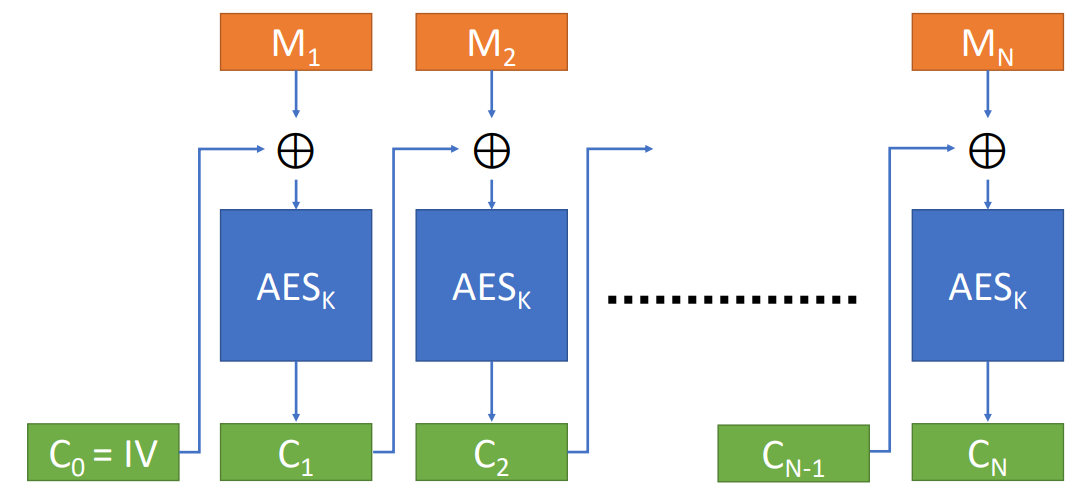
\includegraphics[width=\linewidth]{img/CBC}
  	\caption{CBC mode\label{cbc}}
  \end{figure}
  \begin{figure}[h]
  	\centering
  	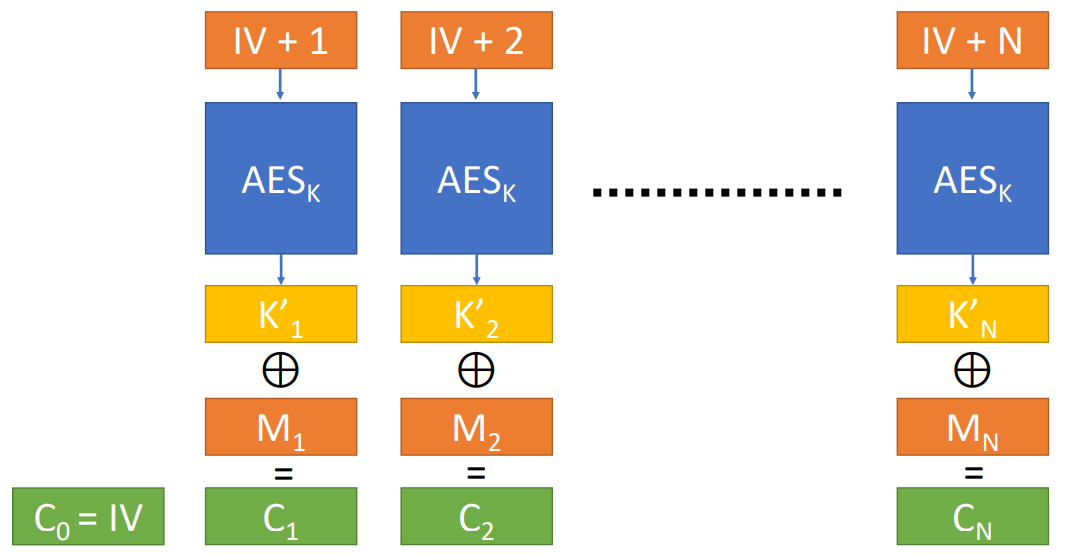
\includegraphics[width=\linewidth]{img/CTR}
  	\caption{CTR mode\label{ctr}}
  \end{figure}
  \item AES er den nuværende standard for block ciphers 
  \item Hovedproblemet ved secret-key systemer er, at både sender og modtager skal kende den samme nøgle før de kan sende data
\end{itemize}

\subsubsection{Public key}
\begin{itemize}
  \item Et public-key kryptosystem består af tre algoritmer $G$, $E$ og $D$ for henholdvis nøgle generation, kryptering og dekryptering
  \begin{itemize}
  	\item Det bruger et par af matchende nøgler en public key $pk$ og en secret key $sk$ 
    \item En bruger $A$ generer nøglerne på hans egen maskine, giver $pk$ væk og beholder $sk$ 
    \item Det skulle gerne være svært at regne $sk$ ud fra $pk$ 
    \item Det skal gælde at $m = D_{sk}(E_{pk}(m))$ 
  \end{itemize}
  \item Det er vigtigt i et public key system, at den samme besked bliver krypteret til noget forskelligt hver gang, da ellers kan en modstander vinde spillet fra definition 5.3 på følgende måde
  \begin{enumerate}
    \item Modstanderen sender en besked $m$ til oraclet
    \item Modstanderen modtager en ciphertekst $c$ fra oraclet
    \item Modstanderen krypterer $c'=E_{pk}(m)$ og konkludere at $c$ er en kryptering af $m$ hvis $c'=c$ og et random $r$ ellers
  \end{enumerate}
  \item Public-key kryptosystemer kan også blive brudt ved hjælp af exhaustive key search 
  \begin{itemize}
  	\item Siden der typisk kun er en privat key der matcher en given public key, så kan modstanderen prøve alle secret-keys indtil han finder den der matcher
    \item Der findes metoder der kan finde en secret key $sk$ fra en public key $pk$, som er meget hurtigere end at prøve alle muligheder
    \item Størrelsen af nøgler til public key systemer er typisk meget større en for secret-key systemer 
  \end{itemize}
\end{itemize}

\subsubsection{RSA}
\begin{itemize}
	\item RSA er et public-key system
  \begin{itemize}
  	\item En public key består af to nummer $n$ og $e$
    \item En private key består af to nummer $n$ og $d$
    \item Nummeret $n$ hedder \textbf{modulus} og er et produkt af to primtal $p,q$ 
    \item Nummerne $e$ and $d$ bliver valgt ud fra primtals faktorerne $p,q$ 
    \item $d$ bliver udregnet som $f(e,p,q)$ for nem udregnelig funktion $f$
    \item Udregning af private key fra public key er lige så svært som at finde $p,q$ fra $n$ 
    \begin{itemize}
    	\item Faktoriseringsproblemet 
    \end{itemize}
  \end{itemize}
  \item Den basale version af RSA som er deterministisk og derfor usikker er som følger
  \begin{itemize}
  	\item Beskeder er numre i intervallet $[0, n]$ 
    \item Man krypter et tal $m$ ved at udregne $c= m^e \mod n$
    \item Man dekryptere en besked ved at udregne $c^d \mod n$ 
    \item De særligt udvalgte $e$ og $d$ sørger for at følgende ligehed er opfyldt
    \begin{equation*}
c^d \mod n = (m^e \mod n)^d \mod n = m
    \end{equation*}
  \end{itemize}   
  \item For at udregne $d$ fra $e,p$ og $q$ er gør man følgende
  \begin{itemize}
  	\item $e$ skal være et tal så den største fælles divisor mellem $e$ og $(p-1)(q-1)$ er $1$ 
    \item $d$ skal udregnes så $d \mod (p - 1)(q - 1) = 1$.
    \item $e$ egenskab sørger for at der altid findes et ordenligt $d$ og bliver typisk skrevet på følgende måde
  \begin{equation*}
  d = e^{-1} \mod (p - 1)(q - 1)
  \end{equation*}

  \end{itemize}
  \item Den eneste måde at bryde RSA på er ved at faktorisere $n$ 
  \begin{itemize}
  	\item De bedste algoritmer kan gøre det på $2^{O(\sqrt[3]k)}$
    \item For at sørger for at disse algoritmer ikke kan bruges skal RSA nøgler være mindst 2000-3000 bits
  \end{itemize}
  \item Siden public key systemer bruger større nøgler en secret key systemer bliver de typisk brugt til at sende en secret key til brug i secret key systemer
\end{itemize}

\newpage

\section{Authentication}
\subsection{Disposition}
\begin{enumerate}
	\item Definition
  \item Secret key
  \begin{itemize}
  	\item Definition
    \item Definition af sikkerhed
    \item Unconditional 
    \item Praktiske Systemer
  \end{itemize}  
  \item Public key
  \begin{itemize}
  	\item Definition
    \item RSA signature
    \item Hash and Sign
  \end{itemize}
\end{enumerate}
\newpage

\subsection{Secret key}
\begin{itemize}
	\item \textbf{Authenticity} man ville være sikker på at det data man modtager er fra senderen 
	\item Et secret key system for authenticity består af tre algoritmer $G, MAC, V$ 
  \begin{itemize}
  	\item $G$ generer en nøgle
    \begin{itemize}
    	\item Dette gøres ved at outputte en random streng af fast længde 
    \end{itemize}
    \item $MAC$ bliver brugt til at autentificere en besked
    \begin{itemize}
    	\item står for \textbf{M}essage \textbf{A}uthentication \textbf{C}ode
      \item tager som input en besked $m$ og en nøgle $k$
      \item giver som output en MAC, $c= MAC_k(m)$ 
    \end{itemize}
    \item $V$ bliver brugt til at verificere en besked
    \begin{itemize}
    	\item $m$ og $c$ bliver sendt til modtageren, som bruge $V$ på inputtet
      \item Resultatet af $V_k(m,c)$ er enter $accept$ eller $reject$
    \end{itemize}
  \end{itemize}
  \item Et authentication scheme skal have den egenskab, at hvis ingen modificerede besked så accepterer modtager altså
\begin{equation*}
V_k(m,MAC_k(m)) = accept
\end{equation*}
  \item \textbf{Definition 6.1} Givet en modstander, som køre i tid mindre en hvad en exhaustive key search vil tage. Så er authentication scheme sikkert hvis der er igen modstander, der kan spille følgende spille og producere en besked $m_0$ and a $MAC$ $c_0$ således at $V_k(m_0,c_0) = accept$ og $m_0 \notin \{m_1, \dots,m_t\}$
  \begin{itemize}
  	\item Modstanderen må givet et hvilket, som helst nummer as beskeder $m_1, \dots, m_t$ og de tilsvarende MACs $c_1, \dots, c_t$ for disse beskeder
    \item Modstanderen må specificere par på formen $(m,c)$ og få fortalt om $c$ er en valid MAC på $m$ 
  \end{itemize}
\end{itemize}

\subsubsection{Unconditional}
\begin{itemize}
	\item En unconditional sikker måde at have MACS på er at senderen og modtager i forvejen bliver enig om et tabel indeholdende for hver besked en random uafhængig valgt $t$ bit MAC
  \item Tabellen fungere som en nøgle
  \item En modstander kan ikke finde en korrekt MAC for en besked udover med sandsynlighed $2^{-t}$ 
  \item Jo længere ``nøglen'' bliver jo flere slags beskeder kan vi have
\end{itemize}

\subsubsection{Pratiske Systemer}
\begin{itemize}
	\item Der er brug for systemer, hvor man kan bruge en lille fast nøgle 
  \begin{itemize}
  	\item Der skal være mindre muligheder for nøglen end der er mulige beskeder 
    \item Dette betyder at en modstander, som har set nogle få valide beskeder og MACs kan finde nøglen ved at bruge exhaustive search  
    \item Dette kan gøre ved at prøve alle muligheder og generer MACs for alle besked der er blevet sendt 
    \item For at sørger for at exhausite key search er uladsiggørlig bruges nøgler af størelse $\geq 128$ 
    \item Størrelsen på MACen kan heller være for lille ellers kan dette også bare bruteforces 
    \begin{itemize}
    	\item 64 bits MACs er ofte brugt
    \end{itemize}
  \end{itemize}
  \item \textbf{CBC-MAC} laver en MAC algoritme fra en hver sikker block-cipher 
  \begin{itemize}
  	\item For at udregner MAC krypter man beskeden i CBC mode og definere MACen til at være det sidste blok af cipherteksten
    \item MACen kan blive verificeret ved at udregne MACen fra den modtagende besked og sammenligne den med den modtagende MAC
    \item Siden den sidste blok af CBC afhænger både af nøglen og hele besked, vil en hvilken som helst ændring i beskeden resultere i en helt anden MAC 
  \end{itemize}
  \item \textbf{HMAC} byger en sikker MAC fra en hvilken sikker kryptografisk hash funktion
  \begin{itemize}
  	\item Hash funktionen \textbf{SHA1} bliver brugt
    \item En hash funktion er hurtig at udregne og producere et fixed størrelses output, men er svær at invertere 
    \item MAC på en besked $m$ og en nøgle $K$ er bare $SHA1(m || K)$ 
  \end{itemize}
  \item MAC algoritmer er generelt lige så hurtige som secret key kryptering
  \begin{itemize}
  	\item De har det samme problem, som er hvordan alle folk får den samme nøgle
  \end{itemize}
\end{itemize}

\subsection{Public key}
\begin{itemize}
	\item Et public-system for authenticity består af tre algoritmer $G, S, V$
  \begin{itemize}
  	\item $S$ bliver brugt til at signe beskeden
    \item $V$ bliver brugt til at verificere den modtagende besked
    \item $G$ outputter et par af nøgler med den rigtige relation mellem dem 
  \end{itemize}
  \item Et party $A$ kan sende en autentificeret besked $m$ ved at beregne $c=S_{sk}(m)$ og sende $m,c$ 
  \begin{itemize}
  	\item En modtager, der kender $A$'s public key $pk$ kan køre $V$ og få resultatet $V_{pk}(m,c)$ som enter er et accept eller eject 
  \end{itemize}
  \item For alle beskeder $m$ og matchende nøgler $pk, sk$ skal vi have
\begin{equation*}
  V_{pk}(m,S_{sk}(m))=accept
\end{equation*}
  \item \textbf{Definition 6.2} En modstander er givet en public key $pk$ 
  \begin{itemize}
  	\item Han kan specificere et hvilket som helst antal af beskeder $m_1, \dots, m_t$ og de valide authenticators  $c_1=S_{sk}(m_1), \dots c_t=S_{sk}(m_t)$ for disse beskeder
    \item Et public key authentication system er sikkeret, hvis en modstander ikke effektivt kan producere en besked $m_0$ og en autheticator $c_0$ således at $V_{pk}(m_0,c_0)=accept$ og $m_0 \notin \{m_1, \dots, m_t\}$
    \item Et systemer der opfylder dette siges at være \textit{``unforgeable under chosen message attack''}
  \end{itemize}
  \item Nøglen skal være længere end i secret key authentication
  \item Alle kan tjekke at senderen er $A$ og derfore er de også kaldet digital signature schemes
  \item Det er vigtigt at modtageren bruge den rigtige public key
\end{itemize}

\subsubsection{RSA signature eksempel}
\begin{itemize}
	\item En usikker måde at bruge RSA med public key $pk=(n,e)$ og private key $sk = n,d$ til at genere signature på følgende måde
  \begin{itemize}
  	\item Antag at beskenden er en numre $m$ i $[0, n-1]$ 
    \item Signaturen på $m$ er $S_{\mathsf{sk}}(m) = m^d \text{ mod } n$
    \item Den specielle måde $d$ og $e$ er valgt på sikre at 
\begin{equation*}
  s^e \text{ mod } n = (m^d \text{ mod } n)^e \text{ mod } n = m 
\end{equation*}
    \item Når man modtager et par $m,s$ kan signaturen tjekkes ved at verificere at $s^e \text{ mod } n = m$
  \end{itemize}
\end{itemize}

\subsubsection{Hash and Sign}
\begin{itemize}
	\item RSA kan ikke bruges direkte som et signature scheme, da det er nemt at finde en besked der overholder $m = s^e \text{ mod } n$
  \item En løsning til hastighed og sikkerhed problemer er en \textbf{kryptografisk hash funktion}, som har følgende egenskaber  
  \begin{itemize}
  	\item Den skal kunne tage en besked af en hvilken som helst længde
    \item Dens output har en fast længde 
    \item Den skal være lige så hurtigt som de bedste secret-key systemer
    \item Det skulle være computational hard at finde en kollision 
  \end{itemize}
  \item En god hash funktion skal have en output længde på mindst 160 bits få at gør det svært at producere en kollision 
  \item For at fixe et signature scheme kan en hash funktion blive brugt sammen med en basic signature scheme fx. RSA og definere en ny signature scheme $S'$ på følgende måde 
  \begin{itemize}
  	\item En signature på en besked $m$ er defineret til at være $S'_{sk}(m) = S_{sk}(h(m))$
    \item Den nye verificering $V'$ på en besked $m$ og en signature $s$  $V'_{pk}(m,s)$ vil udregne $h(m)$ og eksekvere $V_{pk}(h(m),s)$ og accepterer hvis og kun hvis $V$ accepteret den 
    \item Dette fixer hastighedsproblemerne siden hashen er meget mindre en beskeden selv 
    \item Dette fixer sikkerhedsproblemerne siden, at det er svært at finde kollision i en hash funktion
  \end{itemize}
\end{itemize}

\newpage

\section{Key Management and Infrastructure}
\subsection{Disposition}
\begin{enumerate}
	\item Problemet
  \begin{itemize}
  	\item Beskrivelse 
    \item Private key løsning for two parties
    \item Public key løsning for two parties
  \end{itemize}
  \item Key Distribution Centers
  \begin{itemize}
  	\item Definition
    \item Problemer
  \end{itemize}
  \item Certification Authority
  \begin{itemize}
  	\item Definition
    \item Standard certifikat indeholder
    \item Certificate chain og problemer 
  \end{itemize}
  \item Password
  \begin{itemize}
  	\item Valg af password
    \item Brug af password
    \item Opbevaring server og bruger
  \end{itemize}
  \item Hardware
  \begin{itemize}
  	\item Tamper-evident hardware 
    \item Tamper-resistant hardware
  \end{itemize}
  \item Biometrics
  \begin{itemize}
  	\item Beskrivelse
    \item Problemer
  \end{itemize}
\end{enumerate}
\newpage

\subsection{Problem}
\begin{itemize}
	\item Følgende problem skal overvejes, når man løser distribuering af nøgler problem: Et hvilket som helst sikker system parameter har en større risiko for at blive opdaget jo mere det bliver brugt 
  \begin{itemize}
    \item Det er en god praksis, at skifte den nøgle man bruge i regelmæssige intervaller   
  \end{itemize}  
  \item Den almindelige måde at opnå confidentiality (eller authenticity eller begge) i to vejs kommutation mellem $A$ og $B$ er at have en nøgle $K_{AB}$ mellem $A$ og $B$ til at starte med hvilket bliver brugt til at sende nøgler fra $A$ til $B$ 
  \begin{itemize}
    \item For at sende en besked $M$ generer $A$ en tilfældig \texttt{session} nøgle $k$ og sender $E_{K_{AB}}(K), E_k(M)$ til $B$ 
    \item $K$ bliver brugt for flere beskeder men slettede efter et kort stykke tid, dette kunne være når forbindelsen bliver lukket 
    \item Hvis man vil løse problemet for flere bruger skal man bruge en anden løsning siden at antallet af nøgler man skal holde styr gror kvadratisk med antallet af brugere 
  \end{itemize}
  \item En måde at opnå det samme som før er at erstatte den delte nøgle $K_{AB}$ med et public key pair $(sk_B,pk_B)$ generet af $B$ 
  \begin{itemize}
  	\item Kun $B$ kender $sk_B$ og $pk_B$ er offentlig
    \item $A$ kan sende $E_{pk_B}(K)$ til $B$ hvor $K$ er session nøglen 
    \item Ingen secret key skal deles til at starte med 
    \item Man skal stadig sørger for at $A$ bruger den korrekt public key 
  \end{itemize}
\end{itemize}

\subsection{Key Distribution Centers}
\begin{itemize}
	\item \textbf{Key Distribution Centers} er kun baseret på secret key teknologi 
  \begin{itemize}
  	\item Der er kun en KDC og mange bruger 
    \item Enhver brugere $A$ deler en nøgle $K_A$ med KDCen 
    \item Hvis $A$ gerne vil tale med $B$ generer KDCen en nøgle $K$ for sessionen og sender $E_{K_A}(K)$ til $A$ og $E_{K_B}(K)$ til $B$
  \end{itemize}
  \item KDC bliver sjældent brugt siden de har et single point of failure KDCen
  \begin{itemize}
  	\item Alle bruger må have tillid til KDCen fuldstændig, siden KDCen kan dekryptere alt trafikken og forfalske det  
    \item Hvis KDCen er nede, så ryger hele alle de sikre kommutation systemer   
  \end{itemize}
\end{itemize}

\subsection{Certification Authorities}
\begin{itemize}
	\item Et Certification Authority her sit eget nøgle par $(sk_{CA}, pk_{CA})$ 
  \begin{itemize}
  	\item Antag at alle brugere har en ægte kopi af $pk_{CA}$
    \item Enhvert bruger $A$ af systemet må kontakte CA og sende deres public key $pk_A$ til CAen
    \item Den måde $A$ identificerer sig selv på kan ikke være udelukkende kryptografisk   
    \begin{itemize}
    	\item Før $A$ er blevet resterede deler den ikke nogle secret keys med CAen 
      \item CAen kender nogle public keys som den med sikkerhed ved tilhører $A$  
    \end{itemize}
    \item Måder $A$ kan identificere sig selv på 
    \begin{itemize}
    	\item $A$ møder op i person (sker sjældent)
      \item En pin code bliver sendt til $A$ i paper mail og bliver brugt til at logge ind på CAen hjemme siden 
    \end{itemize} 
  \end{itemize}
  \item Hvis en CA accepterer identiteten af en bruger udsteder den et certifikat indeholdende følgende
  \begin{itemize}
		\item En streng $ID_A$
		\item Public keyen $pk_A$
		\item CAens signature $S_{sk_{CA}}(ID_A,pk_A)$ på det andet data    
  \end{itemize}
  \item Når et certifikat er blevet udgivet kan man sætte en sikker forbindelse op 
  \item Hvis bruger tror hans privat key er blevet stjålet, skal det være muligt at rapportere dette
  \begin{itemize}
  	\item Det skal være muligt at tjekke om et givet certifikat stadig er valid via en online service
    \item Et certifikat skal indeholde den periode den er valid i  
  \end{itemize}
  \item Et certifikat er typisk en lang data record der indeholder en masse felter
  \item Man kan bruge et cerification authority til at verificere en anden certification authority fx $Cert_ {CA_1}(CA_2, pk_{CA_2})$
  \item En mere generel måde er at bruge certificate chain, hvilket er en ordnet list af certifikater   
  \begin{itemize}
    \item Det første indgang er et certifikat, hvor $CA_1$ certificere public keyen af den pågældende bruger
    \item Den anden indgang er $CA_2$ der certificere $CA_1$ public key osv indtil det sidste indgang hvor $CA_n$ certificere public keyen for $CA_{n-1}$ 
    \item Certifikat chains begrænsninger 
    \begin{enumerate}
			\item $A$ skal stole på den sidste indgang til det omfang, at han stoler at alle CAer der er involvede i chainen ikke udgiver flaske certifikater     
			\item Den fjerner ikke behovet for at kende den sidste public key til at starte med 
      \begin{itemize}
      	\item I praktiske situationer kommer de krævede nøgler med brugerens software sammen med software der generer nøgler til kryptering og signaturer.   
      \end{itemize}
    \end{enumerate}  
  \end{itemize}
\end{itemize}

\subsection{Password}
\begin{itemize}
	\item Et password er ofte det svageste led i en sikkerhed kæde siden de skal huskes af menneskers 
  \item Der er mindst 4 vigtige sikkerhedaspekter af password sikkerhed  
  \begin{itemize}
  	\item Hvordan bliver et password valgt?
    \begin{itemize}
    	\item Kan en modstander gætte adgangskoden og verificere dette?  
    \end{itemize}
    \item Hvordan er adgangskoden overført mellem bruger og den der verificere password? 
    \begin{itemize}
    	\item Kan en modstander opsnappe adgangkoden mens den bliver sendt?
    \end{itemize}
    \item Hvordan er adgangskoden gemt ved brugeren? 
    \begin{itemize}
    	\item Kan en modstander stjæle adgangskoden fra brugeren? 
    \end{itemize}
    \item Hvordan er adgangskoden gemt ved den der verificerer det? 
    \begin{itemize}
    	\item Kan en modstander stjæle adgangskoden hos den der verificere det? 
    \end{itemize}
  \end{itemize}
\end{itemize}

\subsubsection{Valg og gæt af adgangskode}
\begin{itemize}
	\item Hvis et password er valgt fra karaktersæt af størrelse $C$ og har længde $\ell$ så er der $C^\ell$ mulige adgangskoder 
  \begin{itemize}
  	\item Dette vokser meget hurtigere som en funktion af $\ell$ end en function af $C$
    \item En person kan højest huske 12 karakter siger studier
    \item Mennesker vælger ikke adgangskoder uniformt og derfor er der adgangskoder der er mere sandsynlige end andre  
  \end{itemize} 
  \item Man skal sørger for at der et begrænsede antal login forsøg, så det er svære for en potentiel modstander at gætte adgangskoder
  \begin{itemize}
  	\item Dette kunne gøre det muligt for en modstander at ødelægge availability  
    \item Det er bedre at lade systemet vente noget tid efter nogle fejlet login forsøg og forøg denne tid hver gang 
  \end{itemize} 
\end{itemize}

\subsubsection{Brug og eavesdropping af adgangskode}
\begin{itemize}
	\item Der er mange måder at stjæle en adgangskode på
  \begin{itemize}
  	\item Man kan kigge over ens skulder
    \item Man kan nemt opfange og stjæle en adganskode sendt over LAN
    \begin{itemize}
    	\item Det kunne fx være gratis wifi på en locale café  
    \end{itemize}
    \item Spyware kan blive brugt til at køre kode på offerets computer og opsnappe en adgangskode  
  \end{itemize}
  \item Man skal sørger for at krypterer internettrafikken
\end{itemize}

\subsubsection{Opbevaring og tilegnelse af password - Brugerens side}
\begin{itemize}
	\item Man kan nemt stjæle et password, hvis det er nedskrevet 
  \item Man kan bruge \textbf{social enginering} til at narre bruger til at give deres adgangskode til en
  \begin{itemize}
  	\item Dette kunne fx være et \textbf{phising attack}, hvor man sender en mail til offeret hvor man udgiver sig for at være en anden
  \end{itemize}
\end{itemize}

\subsubsection{Valg og gæt af password - verificereren side}
\begin{itemize}
	\item Nogle gange er det muligt at stjæle adgangskoder på verificerens side 
  \begin{itemize}
  	\item Det kunne fx. være at adgangskoderne var gemt i cleartekst 
    \item Man kan gemme adgangskoderne i en bruger record der indeholder et brugernavn $u$ og $f(pw_u)$ hvor
    \begin{itemize}
    	\item $pw_u$ er adgangskoden for bruger $u$
      \item $f$ er en envejsfunktion hvor det er nemt at udregne $f(pw_u)$ fra $pw_u$ men det er svært at finde den inverse 
      \item $f$ kunne fx være en hashfunktion 
    \end{itemize} 
  \end{itemize}  
  \item Password crackers er programmer der kan bruges til at cracke password filer  
  \begin{itemize}
    \item De bruger dictionaries med mulige password og prøver på at matche adgangskoden i en given password fil
  \end{itemize}
  \item Foranstaltninger imod password crackers  
  \begin{enumerate}
  	\item Man kan lærer brugerne at bruge svære password  
    \item Forsinke angriberen ved at sørger for at funktionen $f$
    \begin{itemize}
    	\item er langsom nok gør antallet af forsøg en angriber kan gennemføre mindre  
      \item er hurtig nok at systemet er effektiv nok
    \end{itemize}
    \item Fjerne single point of failure: mange servere er begynd at hashe adgangkoden sammen med en hemmelig nøgle $K$ på en anden server    
    \begin{itemize}
    	\item En modstander skal både have fat i det hashede password og nøglen $K$
      \item En anden server skal være involverede i verifikation af en adgangskode     
      \item Når brugeren $u$ registrere sit password $pw$ er dette sendt til en hashing sever der udregner $y=f(K,pw)$ og returner denne værdi til autentificeringserveren $(u,y)$ 
      \item Når brugeren kontakter autentificeringserveren, sender den det modtagende passwords $pw'$ og det hashed password $y$ til hashing severen der tjekker hvorvidt $f(K,pw')=y$ eller ikke  
    \end{itemize}
  \end{enumerate}
\end{itemize}

\subsection{Hardware}
\begin{itemize}
	\item Meningen med sikker hardware er at undgå at en modstander får fat i secret keys
  \item Hvis en nøgle er gemt inden i en hardware unit kan en potentiel angriber ikke nemt bryde ind i denne
  \begin{itemize}
  	\item Dette kræver tid og penge
  \end{itemize}
  \item \textbf{Tamper-evident hardware} er hardware der er svært at bryde ind i, men ikke umulig 
  \begin{itemize}
  	\item Fx. chip kort
    \item Kommer typiske med deres egen computer
    \item Disse enheder skal programmeres forsigtigt med sådan de ikke afsløre noget om nøglen
    \item De bliver typisk brugt for two-factor authentication
    \begin{itemize}
    	\item En bruger skal først autentificere sig selv med et password og derefter checke hvorvidt bruger han en bestemt hardware unit 
      \item En secret key $K$ bliver typisk gemt inden i enheden
      \item En verificere giver enheden en challenge $c$ (nonce), som brugeren giver til hardware enheden og returnerer $R(K,c)$
      \begin{itemize}
      	\item Man kryptere typisk $c$ og $K$
        \item Replay angreb virker ikke siden det er en unik opgave hver gang 
        \item Det kan stadig blive angrebet af realtime phising
      \end{itemize}
    \end{itemize}
  \end{itemize}
  \item \textbf{Tamper-Resistant hardware} er meget svære at bryde ind i end tamper evident hardware
  \begin{itemize}
  	\item Ikke engang en stor virksom med ekspert viden kan bryde ind i sådan en enhed
    \item Nogle af dem har deres egen CPU, hukommelse og battery og kan gøre alle de normale kryptografisk algoritmer
    \item Bliver brugt af CA's til at gemme deres private keys
  \end{itemize}
\end{itemize} 

\subsection{Biometrics}
\begin{itemize}
	\item \textbf{Biometrics} bruger forskellige fysiske karakteristikker af personen der prøver at få adgang
  \begin{itemize}
  	\item Man kan fx skanne sit fingeraftryk, øje, ansigt eller høre til ens stemme
    \item Det største problem ved dette er konverteringen til digital og sammenligning med dete
    \begin{itemize}
    	\item System skal være tolerant nok til at acceptere de rigtige bruger
      \item System skal være restriktivt nok til at afvise dem der prøver at snyde 
    \end{itemize}   
  \end{itemize}  
  \item Det giver bedre access control for ens private sikkerhedsnøgle 
  \item Man skal tænke over hvordan afmålingerne bliver gemt 
\end{itemize} 

\newpage

\section{Network Security Mechanisms}
\subsection{Disposition}
\begin{enumerate}
	\item Authenticated key exchange
  \begin{itemize}
    \item Problem
  	\item Definition
  \end{itemize}
  \item SSL/TLS
  \begin{itemize}
    \item Beskrivelse
  	\item Protokol
    \item Argumentation for sikkerhed
  \end{itemize}
  \item Diffie Hellman Key Exchange og forward secrecy 
  \begin{itemize}
  	\item Definition af forward secrecy
    \item Diffie Hellman Protokol
    \item Argumention af forward secrecy
    \item Problemer
  \end{itemize}
\end{enumerate}
\newpage

\subsection{Authenticated key exchange}
\begin{itemize}
	\item Threat modelen er at modstanderen kan se og modificere alt kommunikation  
  \item $A$ og $B$ vil gerne etablere en sikker forbindelse over internettet de har begge to et certifikat der indeholde public keys $pk_A$ og $pk_B$  
  \item En \textbf{authenticated key exchange} protocol er en protocol for to parties $A$, $B$ 
  \begin{itemize}
  	\item Begge parties starter protokollen med en intension om a etablere en nøgle med et andet party  
    \item I slutning, outputter hvert party enten ``reject'' eller ``accept'' sammen med en nøgle
  \end{itemize}
  \item Man siger at authenticated key exchange er sikker hvis den overholder de føgende tre betingelse
  \begin{itemize}
    \item \textbf{Agreement:}
    \begin{itemize}
      \item Antag at $A$ gerne vil tale med $B$ og $B$ gerne vil tale med $A$ 
      \item Antag at begge parties accepterer og $A$ outputter nøglen $K_A$ og $B$ outputter $K_B$. Så skal der gælde at $K_A = K_B$  
    \end{itemize}
    \item \textbf{Secrecy} og \textbf{Authentication}: hvis $A$ gerne vil tale til $B$, og accepterer, så skal $B$ have deltaget i protokollen og hvis $B$ også accepterer
    \begin{itemize}
    	\item Så ville han gerne tale til $A$   
      \item Modstanderen kender ikke nøglen $K$ som $A$ outputter
      \item Dette samme holder for $B$ 
    \end{itemize}
    \item \textbf{Freshness:} hvis $A(B)$ følger protokollen og acceptere, så er det garanteret at den nøgle $K$ der bliver outputtede er en ny nøgle   
    \begin{itemize}
    	\item Altså har protokollen valgt en tilfældig nøgle
    \end{itemize}
  \end{itemize}
\end{itemize} 

\subsection{SSL/TLS}
\begin{itemize}
  \item SSL er en af de mest almindelige løsning for authenticated key-exchange der bliver brugt i dag
  \begin{itemize}
    \item Denne bruger digitale signaturer sammen med kryptering 
	  \item SSL bliver blandt andet brugt til at sætte sikre HTTP forbindelser op 
    \item Det er placerede mellem applikations og TCP/IP transport laget 
    \begin{itemize}
    	\item Den transportere dataen i TCP/IP pakker 
    \end{itemize}
    \item I dens normale form kræver den at både severen og klienten har et public-key certifikat og de tilsvarende private keys   
    \begin{itemize}
    	\item Det er også muligt at lave en one-sided SSL, hvor det kun er serveren der har et certifikat  
    \end{itemize}
    \item SSL består af flere protokoller hvor en af dem er \textbf{Handshake Protokol}, som gør den authencated keyexchange
    \begin{itemize}
    	\item Dette betyder også at sikkerhed af denne ikke giver sikkerhed af hele SSL konstruktionen
      \item Den beskrevende del er en simplificering af den rigtige protokol 
    \end{itemize}
  \end{itemize}
\end{itemize}
\begin{framed}  
  \begin{center}  
     \textbf{SSL key exchange} 
  \end{center}
  \begin{enumerate}
  	\item $C$ sender en ``hej'' besked indeholdende $n_c$ 
    \item $S$ sender en nonce $n_s$ og dets certifikat $Cert_s$
    \begin{itemize}
    	\item Certifikatet indeholder public key $pk_s$ af $S$ 
    \end{itemize}
    \item $C$ verificerer $Cert_s$ og vælger en pre master secret $pms$ tilfældigt 
    \begin{itemize}
     	\item $C$ sender $E_{pk_s}(pms)$ til $S$ sammen med sit certifikat $Cert_C$ og dens signature $sig_c$ af konkatenation af $n_c$, $n_s$ og $E_{pk_s}(pms)$ 
    \end{itemize}
    \item $S$ verificere $Cert_C$ og $sig_C$, hvis OK så dekryptere den $pms$ 
    \item $S$ sender til $C$ en ``færdige'' besked der indeholder en MAC på alle beskeder han har sent og modtaget i denne instans af protokollen, hvor $pms$ er secret key  
    \item $C$ verificere MACen og hvis OK returner sin egen ``færdige'' besked, med en MAC på alle beskeder sent og modtaget op til dette tidpunkt   
    \begin{itemize}
    	\item $S$ verificere dette når det bliver modtaget
    \end{itemize}
    \item Begge parties udleder et set af nøgler ud fra $n_s$, $n_s$ og $pms$ til secret key authentication og kryptering til den efterfølgende data kommunikation
    \begin{itemize}
    	\item Dette bliver typisk gjort med en hash funktion
    \end{itemize}
  \end{enumerate}
\end{framed}
\begin{itemize}
	\item Den sidste del af protokollen sørger for at $S$ autentificere sig selv ved at vise at den kan den har fortaget de samme transaktioner
  \begin{itemize}
  	\item Dette beviser, at den kunne udregne $pms$ og derfor kender $sk_s$  
    \item Klienten autentificere sig selv ved at kunne signe beskeden indeholdende krypteringen af $pms$ 
    \item MACing af det hele sørger for at en potentiel angriber ikke har ændret nogle beskeder og derfor at $S$ og $C$ har set de samme beskeder  
    \item Den sørger for at angriber kun kan se beskeder og ikke ændre dem
  \end{itemize}
  \item Argumentation for sikkerhed
  \begin{itemize}
  	\item \textbf{Agreement} holder siden begge parties kender samme $n_s$, $n_c$ og $pms$ 
    \begin{itemize}
    	\item Hvis en af dem var forskellige ville step 5. eller 6. have fejlet 
    \end{itemize}
    \item \textbf{Secrecy} og \textbf{Authentication} holder siden   
    \begin{itemize}
    	\item Modstanderen kender ikke $pms$, hvis han gjorde dette skulle han kunne $E_{pk_s}(pms)$ hvilket vil betyder at han kendte secret keyen
      \item De er sikker på at hinanden har deltaget i protokollen og gerne vil tale med dem siden eller ville 5 eller 6 have fejlet  
    \end{itemize}
    \item \textbf{Freshness} kommer af, at $pms$ kræves at være valgt tilfældigt
  \end{itemize}
\end{itemize}

\subsection{Diffie Hellman Key Exchange og forward secrecy}
\begin{itemize}
	\item \textbf{Forward secure} betyder at sikkerheden af en session ikke kan bliver comprised selvom modstanderen stjæler ens secret key engang i fremtiden  
  \begin{itemize}
  	\item En variant af SSL handshake, der er baseret på RSA er ikke forward secure
    \item En variant af SSL handshake, der er baseret på Diffie-Hellman er forward secure
  \end{itemize}
  \item Diffie-Hellman Key Exchange bruger i sin basic form 
  \begin{itemize}
  	\item Et aritmetik modulo med et primtal $p$ 
    \item Et nummer $g$ i intervallet $0$ til $æ-1$ bliver valgt en gang for alle
    \item Når en client $C$ og en server $S$ gerne vil udveksle nøgler bliver den beskrevende protokol brugt 
  \end{itemize}
\end{itemize}

\begin{framed} 
  \begin{center}  
     \textbf{Diffie-Hellman key exchange} 
  \end{center}
  \begin{enumerate}
  	\item $C$ vælger et tilfældigt tal $a$ og sender $g^a \text{ mod } p$ sammen med hans certifikat til $B$ 
    \item $S$ vælger et tilfældigt tal $b$ og sender $g^b \text{ mod } p$ sammen med hans certifikat til $A$ 
    \item $C$ udregner $(g^b \text{ mod } p) ^a \text{ mod } p$ og $S$ udregner $(g^a \text{ mod } p) ^b \text{ mod } p$
    \begin{itemize}
    	\item De udregnede værdier er ækvivalente siden de begge er lig med $g^{ab}  \text{ mod } p$ og denne værdi kan bruges som nøgle 
    \end{itemize}
    \item C signer alle beskeder han har set og sender signaturen til $S$
    \begin{itemize}
    	\item S signer også alle de beskeder han har set og sender signaturen til $C$  
    \end{itemize} 
    \item Begge parties verificeret de modtagende signature mod de beskeder de har set og public key fra det andet party
    \begin{itemize}
    	\item Hvis alting er OK, er protokollen succesful 
    \end{itemize}
  \end{enumerate}
\end{framed}
\begin{itemize}
	\item Hvis $p$ er stor nok, mener man at infeasible at udregne fra information sendt nøglen   
  \begin{itemize}
  	\item Kaldet \textbf{Diffie-Helman problemet}
  \end{itemize}
  \item Problemer med Diffie-Helman key exchange
  \begin{itemize}
  	\item Der er en algoritme kendt som Index Calculus der løser Diffie-Helman problemet og derfor bryder protokolen
    \begin{itemize}
    	\item Den kan gøre det effektivt efter en lang og ineffektive preprocessing, som kun afhænger af primtallet $p$ 
      \item Man kan løse det på forskellige måde
      \begin{itemize}
      	\item Man kan bruge et nye primtal for protokolen, ikke for hver instans af protokolen men med små regulær intervaller  
        \item Man kan bruge et andet setup, som er den protokol der er baserede på Elliptic Curve kryptografi i steddet for aritmetiks modulo prime
      \end{itemize}
    \end{itemize}
  \end{itemize}
\end{itemize}
\newpage

\section{System Security Mechanism}
\subsection{Disposition}
\begin{enumerate}
	\item Trusted computing base
  \begin{itemize}
  	\item Definition af system security
    \item Definition af trusted computing baase
  \end{itemize}
  \item Security policies
  \begin{itemize}
  	\item Definition
    \item Modeller
    \begin{itemize}
    	\item Definition
      \item Lattice definition
      \item Lattice som model 
      \item Bell-Lapadula 
      \item Biba modelen
    \end{itemize}
  \end{itemize}
  \item Access control
  \begin{itemize}
  	\item Access control matrix model 
    \item Organiseringen af matricen
    \item Dynamisk access control matrix
    \begin{itemize}
    	\item Måder at opdaterer den på 
      \item Definition af kommando og uafgørlighed 
    \end{itemize}
  \end{itemize}
\end{enumerate}
\newpage
  
\subsection{Trusted computing base}
\begin{itemize}
	\item \textbf{System Security} er mekanismer der prøver at stoppe eksterne angribere fra at komme end i systemet 
  \begin{itemize}
  	\item Dette gælder også angreb fra parties, der allerede er en del af system
    \item Man skal sørger for at hvis et party vil have adgang til en del af systemet, at partiet kun får afgang, hvor det er er okay med hensyn til vores security policy 
    \item Hvis ens adgang bliver afvist, skal det ikke være muligt at få adgang alligevel
  \end{itemize}
  \item En \textbf{trusted computing base} er en del af systemet der ikke kan bliver modificeret af angribere 
  \begin{itemize}
  	\item Det kan blive etablerede ved hjælp af hardware og eller software afhængig af threat modellen    
    \item Det er ofte en del af operativ systemets kernel
    \item Den består af en eller flere hardware enheder 
  \end{itemize}
\end{itemize}

\subsection{Security Policies}
\begin{itemize}
	\item \textbf{Security Policy definition}
  \begin{itemize}
    \item Den indeholder en beskrivelse af systemet, der bliver anvendt på 
  	\item Den beskriver de security objectives, man gerne vil opnå 
    \item Den kan have forskellige former
    \begin{itemize}
    	\item Det kan være en specifikation af hvad forskellige enheder må gøre og ikke gør
      \item Det kan være en specifikation at hvilke events, man vil håndtere når systemet kører  
    \end{itemize}
    \item En policy indeholde en beskrivelse på højt niveau hvad for nogle metoder der vil blive brugt til at håndhæve security objectives 
    \item Systemet skal sørger for at ingen enheder kan gøre noget de ikke har lov til eller at intet event sker som man ikke tolerer 
    \item Det er det sted, hvor man formulere de regler som TCB skal håndhæve 
  \end{itemize}
\end{itemize}

\subsubsection{Security Policies modeller}
\begin{itemize}
	\item \textbf{Modeller for Security Policies} er abstrakte beskrive af måde at designe en security policy på  
  \begin{itemize}
  	\item er ofte ikke en beskrivelse af et konkret system
    \item adressere ofte bestemte threat modeller 
  \end{itemize}
  \item En security policy er derfor typisk en realisation af en model med hensyn til et bestemt system 
  \begin{itemize}
  	\item kan dog også være baseret på mere en model  
  \end{itemize}
  \item En \textbf{lattice} indeholder et endeligt set $S$ sammen med en relation $\leq$. For hvilke som helst elementer $a,b,c \in S$ skal det holde at
  \begin{itemize}
  	\item $a \leq a$
    \item $a \leq b$ og $b \leq a$ medføre $a=b$  
    \item $a \leq b$ og $b \leq c$ medføre $a \leq c$ 
  \end{itemize}
  \item For at $S, \leq$ er en lattice så er det krævet at for hvilket som helst elementer $a,b \in S$, at der gælder 
  \begin{itemize}
  	\item Der eksistere et \textbf{greatest lower bound} for $a,b$ 
    \begin{itemize}
    	\item Der eksister et $c \in S$ således at $c \leq a$, $c \leq b$ og for et ethvert andet element $c'$, med denne egenskab gælder det $c' \leq c$ 
    \end{itemize}
  	\item Der eksistere et \textbf{greatest upper bound} for $a,b$ 
    \begin{itemize}
    	\item Der eksister et $d \in S$ således at $a \leq d$, $b \leq d$ og for et ethvert andet element $d'$, med denne egenskab gælder det $d \leq d'$  
    \end{itemize}
  \end{itemize}
  \item Man kan tænke på $S$ som et sæt af privilegier eller rettigheder en bruger har i et system 
  \begin{itemize}
  	\item $a \leq b$ betyder at med rettigheder $b$ har man mindst lige så mange rettigheder som $a$ 
    \item Nogle rettigheder kan ikke sammenlignet sidden det ikke er et krav at $\leq$ er defineret for alle par 
  \end{itemize}
  \item Der er mindst to måde at bruge lattice modellen til at organisere et security policy 
  \begin{enumerate}
  	\item Definere \textbf{subjekt} til at være alle brugere og processer i systemet 
    \begin{itemize}
    	\item Et \textbf{objekt} er resourcer, filer, hardware devices osv.
      \item Alle subjekter og objekter er klassificeret således de har en position is latticen  
      \item Et subjekt $s$ med klassifikation $C(s)$ må kun køre en given operation på objekt $o$ med klassifikation $C(o)$ hvis og kun hvis $C(s) \leq C(o)$ eller $c(o) \leq c(s)$ 
    \end{itemize}
    \item Man kan tildele en position i latticen til forskellige dele af systemet 
    \begin{itemize}
    	\item Information må kun komme fra position $a$ til position $b$ hvis $a \leq b$ 
      \item De højre positioner er mere hemmelig
      \item Fokus er confidentiality
      \item Hvis den fokuserede på authenticity, så var de højre positioner de mere pålidlige dele af systemet
      \begin{itemize}
      	\item Information må kun komme fra $a$ til $b$ hvis $a \leq b$ 
      \end{itemize}
    \end{itemize}
  \end{enumerate}  
  \item \textbf{Bell-Lapadula} modelen er som følger
  \begin{itemize}
  	\item Der er et antal sikkerhed niveauer, der er linært ordered 
    \item Modellen har følgende regler
    \begin{itemize}
    	\item \textbf{No read up:} Et subjekt $s$ må kun læse et objekt hvis $C(s) \geq C(o)$ 
      \item \textbf{No write down:} Et subjekt $s$ må kun skrive til at objekt $o$ hvis $C(s) \leq C(o)$ 
    \end{itemize}
    \item Information må ikke komme fra højre niveauer til laver niveauer 
    \item Dette er ikke et særligt fleksibel system og kan være svært at håndtere i praktisk
  \end{itemize}
  \item \textbf{Biba modelen} fokusere på integritet 
  \begin{itemize}
  	\item De højere niveauer indeholder det mest pålidelige information
    \item Modellen har følgende regler
    \begin{itemize}
    	\item \textbf{No read down:} Et subjekt $s$ må kun læse et objekt hvis $C(s) \leq C(o)$ 
      \item \textbf{No write up:} Et subjekt $s$ må kun skrive til at objekt $o$ hvis $C(s) \geq C(o)$ 
    \end{itemize}
    \item Information må ikke komme fra lavere niveauer til højere niveauer  
  \end{itemize}
\end{itemize}

\subsection{Access control}
\begin{itemize}
	\item Det er generelt antaget, at når en bruger gerne vil eksekvere en operation på et objekt, så er det muligt at verificere identiteten af brugeren og finde ud af hvilket rettigheder og privilegere brugeren har   
  \begin{itemize}
  	\item At tjekke en brugers indentitet er et teknisk problem  
    \item At finde ud af hvilke rettighed en bruger har er et helt andet problem  
    \begin{itemize}
    	\item Dette kan typisk blive udregnede fra en brugers identitet og security policy  
      \item Det er vigtig, at denne information er organiserede på en ordentlig møde, siden det typisk skal gøres, mens en bruger venter på adgang 
    \end{itemize}
  \end{itemize}
  \item En generisk møde at organisere rettighederne på bliver kaldt en \textbf{Access control matrix}
  \begin{itemize}
  	\item Det er en matrix $A$ med en række for hvert subjekt $s$ og en søjle for hvert objekt $o$ 
    \item Et entry $A[s,o]$ indeholder en list af alle operationer $s$ må gøre på $o$ 
    \item I realistiske systemer er det ikke praktisk at gemme helle matricen på en central location
  \end{itemize}
  \item I praktis er der to forskellige måde at organisere en Access control matrix     
  \begin{enumerate}
  	\item \textbf{Access Control List} her gemmes sammen med filen, dens column i matricen
    \begin{itemize}
    	\item Denne liste gør det nemt at sige for en given objekt hvem der har adgang 
      \item Det er meget svære at sige hvad et given subjekt kan gøre
      \item Dette er cirka den møde UNIX systemet gør det 
    \end{itemize}
    \item \textbf{User Capabilities} her gemmer hvert subjekt, dens række i matricen 
    \begin{itemize}
    	\item Dette gør det nemt at se hvad en given bruger kan gøre
      \item Det er svære at finde ud af hvem der har adgang til et given objekt 
      \item Windows bruger denne cirka denne
    \end{itemize} 
  \end{enumerate}
  \item I større systemer splitter man typisk brugerne ind i predefineret gruppe
  \begin  {itemize}
  	\item Siden ellers bliver ACLen for lang
    \item Den siger kun hvad subjekter fra hver gruppe kan gøre
  \end{itemize}
\end{itemize}

\subsubsection{Dynamisk Access control matrix}
\begin{itemize}
	\item Der er to forskellige metoder for at opdatere en Access control matrix 
  \begin{enumerate}
  	\item \textbf{Mandatory access control:} subjekter kan ikke ændre matricen
    \item \textbf{Discretionary access control:} subjekter har rettighed til at opdatere matricen eller dele af den
  \end{enumerate}
  \item Givet at en access control matrix kan ændre sig med tid er det normalt at spørge hvilke typer af informationer flows det acceptere 
  \item Harrison, Ruzzo and Ullmani har studeret dette spørgsmål i en formel model, her er nogle primitive operationer tilladt på access control matricen $A$   
  \begin{itemize}
  	\item Lav/slet subjekt $s$
    \item Lav/slet objekt $o$ 
    \item Tilføj/fjern adgangsrettighed $r$ fra $A[s,o]$
  \end{itemize}
  \item Det er antaget at der er et fast antal rettigheder
  \item En kommando har følgende form
\begin{lstlisting}[mathescape=true]
Command com(parameter-list)
$r_1$ is in $A[s_1,o_1]$
$\cdots$
$r_n$ is in $A[s_n,o_n]$
list of primitive operations
\end{lstlisting}
  \item Listen af de primitive operation vil blive eksekveret hvis alle de angivende konditioner i den første del er opfyld
  \begin{itemize}
  	\item Alle rettigheder, subjekter og objekter, der bliver referet til i specifikationen af \texttt{com} er taget fra parameter listen
    \item Hvis man er givet et fast set af kommandoer $com_1, com_2, \dots, com_t$ og en initel access control matrice for en given rettighed $r$ kan man spørge hvorvidt der eksisterede et set af kommandoer der vil transformere $A$ til matricen $A'$ hvor $r \in A'[s,o]$ for nogle $s,o$ men hvor $r \notin A[s,o]$  
    \begin{itemize}
    	\item Hvis svaret er nej er $A$ sikker med hensyn til $r$  
    \end{itemize}
    \item Hvis kommandoer indeholder mere end en operation, er det uafgørligt hvorvidt $A$ er sikker med hensyn til $r$   
    \item Hvis de kun indeholder en enkelt primitiv operation, så er det afgørlig
    \item Hvis der er et fast antal subjekter og objekter så er det afgøreligt hvorvidt $A$ er sikker med hensyn til $r$ 
  \end{itemize}
\end{itemize}
\newpage

\section{Threats and Pitfall}
\subsection{Disposition}
\begin{enumerate}
	\item STRIDE
  \begin{itemize}
  	\item Karakterisering af det man gerne vil opnå
  \end{itemize}
  \item X.800
  \begin{itemize}
  	\item Primært til netværkangreb
    \item Karakterisere hjælpemidler man har gjort brug af
    \item Passive attacks
    \item Active attacks
  \end{itemize}
  \item EINOO
  \begin{itemize}
  	\item Who
    \item Where
  \end{itemize}
  \item TPM
  \begin{itemize}
  	\item Hvad gjorde angrebet muligt?
  \end{itemize}
  \item Angrebseksempler
  \begin{itemize}
    \item IBM 4758
    \begin{itemize}
    	\item Beskrivelse
      \item Karakterisering
    \end{itemize}
  	\item Heart Bleed Bug
    \begin{itemize}
    	\item Beskrivelse
      \item Karakterisering
    \end{itemize}
    \item The Unicode Exploit
    \begin{itemize}
    	\item Beskrivelse
      \item Karakterisering
    \end{itemize}
  \end{itemize}
\end{enumerate}

\newpage

\subsection{STRIDE} 
\begin{itemize}
	\item STRIDE er en måde at karakterisere et attack på baseret på hvad de gerne vil opnå 
  \begin{itemize}
    \item \textbf{Spoofing Identity:} resulterer i at attackeren kan udgive sig for at være brugeren   
    \item \textbf{Tampering:} resulterer i at attackeren kan manipulere data uden at blive opdaget
    \item \textbf{Repudiation:} resulterer i at attackeren kan benægte noget han rent faktisk gjorde
    \item \textbf{Information Disclosure:} resultere i at attackeren har adgang til data han ikke skulle kunne se   
    \item \textbf{Denial of service:} resulterer i at attackeren kan benægte andre adgang til system
    \item \textbf{Elevation of privilege:} resultere i at attackeren kan få flere en rettigheder en han skulle have
  \end{itemize}
  \item Det samme attack kan have flere forskellige effekter på samme tid 
\end{itemize} 

\subsection{X.800}
\begin{itemize}
	\item Man prøver at karakterisere de hjælpemidler en attacker har gjort brug af
  \item X.800 standarden har to hovedtyper af angreb på netværkstransmissioner  
  \begin{itemize}
  	\item \textbf{Passive Attacks:}
    \begin{itemize}
    	\item \textbf{Eavesdropping:} Attackeren lytter og kigger på det information der bliver sendt
      \item \textbf{Traffic Analysis:} Attackeren kigger kun hvem der sender til hvem og hvor meget der bliver sendt
    \end{itemize}
    \item \textbf{Active Attacks:}
    \begin{itemize}
    	\item \textbf{Replay:} Attackeren gensender en gammel besked
      \item \textbf{Blocking:} Attackeren stopper en besked fra at blive modtaget 
      \item \textbf{Modification:} Attackeren ændre dataen der bliver sendt og indsætter en ny besked
    \end{itemize}
  \end{itemize}
  \item Passive attacks er svære at opdage   
  \begin{itemize}
  	\item Man kan bruge kryptering imod eavesdropping
    \item Kryptering kan ikke stoppe traffic analysis
    \begin{itemize}
    	\item Man kan sende en besked til mange parties for at skjule modtageren
      \item Randomisere længden af beskeden for at skjule den faktiske beskeds længde 
      \item Man kan bruge stenografi
    \end{itemize}
  \end{itemize}
  \item Aktive attacks er nemme at opdage
  \begin{itemize}
    \item Man kan bruge MACs, signaturer, sekvensnumre på beskeder osv.
  \end{itemize}
\end{itemize} 

\subsection{EINOO}
\begin{itemize}
	\item \textbf{Who} 
  \begin{itemize}
  	\item \textbf{External attackers:} nogle der ikke er brugere af systemet
    \item \textbf{Insiders:} nogle der er registreret som bruger og har noget adgang til at starte med
  \end{itemize}
  \item \textbf{Where} 
  \begin{itemize}
  	\item \textbf{Network attacks:}
    \begin{itemize}
    	\item Modstanderen kan kun lytte og måske modificere internet traffiken
      \item Der er normalt umuligt at undgå at disse angreb bliver prøvet, men kan næsten altid blive afhjælpet med kryptografi   
    \end{itemize}
    \item \textbf{Off-line attacks:}
    \begin{itemize}
    	\item Modstanderen får uautoriseret adgang til information, der er permanent gemt på systemet  
      \item Han kan stjæle og/eller modificere informationen 
      \item Dette kan fx være at stjæle en password database fil
      \item Det er svære en netværkangreb siden man skal komme forbi systemets access control  
      \item Kryptografisk beskyttelse af data er en måde at beskytte mod dette 
      \begin{itemize}
      	\item De kryptografiske nøgler skal ikke gemmes samme sted
      \end{itemize}
    \end{itemize}
    \item \textbf{On-line attack:}
    \begin{itemize}
    	\item Modstanderen bryde ind i systemet imens programmer, der håndterer sensitiv information, kører    
      \item Man kan fx læse secret keys fra ram
      \item Svære end off-line attack at udføre
      \item Modstanderen skal fuldstændig ødelægge access control
      \item Dette kan kun beskyttes ved at have forskellige dele af systemet beskyttet på forskellige måder 
    \end{itemize}
  \end{itemize}
  \item Denne model kan være brugbart, når man designer threat modeler for konkrete systemet  
\end{itemize} 

\subsection{TPM}
\begin{itemize}
	\item En måde at karakterisere angreb på i forhold til hvad der gjorde angrebet muligt  
  \begin{itemize}
  	\item \textbf{Threat model:} Angrebet var muligt på grund af threat modellen ikke var komplet 
    \begin{itemize}
    	\item Et angreb man ikke tænkte på var relevant 
    \end{itemize}
    \item \textbf{Policy:} Angrebet var muligt fordi specification af security policy udtrykker noget andet end det man mente
    \item \textbf{Mechanism:} Angrebet var muligt, da sikkerhedmekanismen kunne omgås 
  \end{itemize}
\end{itemize} 

\subsection{Angrebseksempler}
\subsubsection{IBM 4758}
\begin{itemize}
	\item Det skete på et hardware unit 
  \begin{itemize}
  	\item Den gør således at attackeren ikke kan læse data eller modificere den kode, som den kører 
    \item Security policien var på det API, der specificeret hvad boksen kunne   
    \item Nogle PhD studerende fandt en måde, man kunne bruge API til at extracte dens secret keys, uden at have tilladelse til det 
    \end{itemize}
  \item Hovedgrunden til at angrebet var muligt var, at boksen både tillod DES encryption med en enkelt 56-bit DES nøgle og two-key triple DES hvor to nøgler en konkataneret til at forme en 112 bit nøgle  
  \begin{itemize}
  	\item 56-bit er ikke sikkert mere og var der kun for backward capability 
    \item Man kan få boksen til at vælge 56 bit DES nøgle $K_0$ og krypterer data under denne nøgle 
    \begin{itemize}
    	\item Man kan effektivt finde den nøgle med exhaustive key search på plainteksten og cipherteksten
    \end{itemize}
    \item Man kan få boksen til at transportere en 112 bit nøgle $K$ ved at splitte nøglen i to dele $K_1$ og $K_2$ hvor $K = K_1 \oplus K_2$ 
    \begin{itemize}
    	\item Man vil så sende nøgle delen via to forskellige kanaler, fx transpoterede af to forskellige personer, som så manuelt inputter nøglen
      \item Det bliver gjort af funktionen \textit{Compine Key Parts} 
      \item Det er antaget, at de to personer ikke snakker sammen
    \end{itemize}
    \item Når en nøgler $K$ er blevet udregnet og hvis der er blevet defineret til at være en key encryption key, så kan man få boksen til at bruge $K$ til en \textit{Export Key} operation, som outputter $E_K(K')$ 
    \begin{itemize}
    	\item $K'$ kan være alle nøgler gemt på boksen
    \end{itemize}
  \end{itemize}
  \item Problemet opstår siden at der ikke er nogen separation mellem brugen af single og dobbelt længde nøgler
	\item Man kan få boksen til at lave en dobbelt længde nøgle ved konkatanere en enkelt længde nøgle med sig selv
  \begin{itemize}
  	\item Dette svarer til at krypter med en enkelt længde nøgle
    \item Dette bliver kaldt en \textit{replicated key}
  \end{itemize}
  \item Angrebet forgår på følgende måde med brug af en person
  \begin{enumerate}
  	\item Få boksen til at lave en single længde nøgle $K_0$ 
    \begin{enumerate}
      \item Få boksen til at krypterer noget data $M$ under $K_0$ 
    	\item Bruge cipherteksten $C$ til at finde nøglen ved brug af exhaustive key search
    \end{enumerate}
    \item Få boksen til at forme en tilfældig dobbelt længde $K_2$ med \textit{replicated dele}
    \begin{itemize}
    	\item Få boksen til at eksportere $K_0$ under $K_2$     
      \item Dette er okay, siden $K_0$ ikke bedre end $K_2$  
      \item $K_2$ skal defineres som en encryption key, som kan bruges til at eksportere andre nøgler
      \item $K_2$ kan ikke bruges til at kryptere data
    \end{itemize}
    \item Man bruger $E_{K_2}(K_0)$ produceret i det forrige step til at finde $K_2$ vha. exhaustive search 
    \item Manuelt skriv en non-replicated nøgle del $K_1$
    \begin{itemize}
    	\item Man udgiver sig for at være i gang med at transportere en nøgle
    \end{itemize}
    \item Kald Combine key parts for a producere $K=K_1 \oplus K_2$ 
    \item $K$ er en nu 112 bit, som nu kan bruges til at eksportere alle nøgler 
    \begin{itemize}
    	\item Attackeren kender $K$ og kan derfor finde ud af alle nøgler i boksen 
    \end{itemize}
  \end{enumerate}
  \item Dette angreb er karaketeriserede på følgende måde  
  \begin{itemize}
	  \item \textbf{STRIDE:} 
    \begin{itemize}
  		\item Information Disclosure
  		\item Spoofing Identity
  		\item Elevation of privilege
  		\item Repudiation (maybe)
    \end{itemize}
  	\item \textbf{X.800:} Modification - Den der er tættest på 
    \begin{itemize}
    	\item Man bruger funktioner i API, men ikke på den måde det er tænkt, at de skal bruges
    \end{itemize}
    \item \textbf{EINOO:}
    \begin{itemize}
    	\item \textbf{Who:} Insiders
      \item \textbf{Where:} Off-line Attack 
    \end{itemize}
	  \item \textbf{TPM:} Policy 
  \end{itemize}
\end{itemize}
\subsubsection{The Heart Bleed Bug}
\begin{itemize}
	\item Skete i OpenSSL som er open-source software der implementerer SSL/TLS
  \item Klienten kunne tjekke at serveren stadig var i live  
  \begin{itemize}
  	\item Dette blev gjort ved at sende en nonce og den længde til serveren også vil severen returnere den samme nonce 
  \end{itemize}
  \item Serveren har i RAM både gemt noce og længden $\ell$  
  \begin{itemize}
    \item Dette ville producerer beskeden til klienten ved at læse $\ell$ karaktere fra arrayet 
  \end{itemize}
  \item Hvis en ond klien sendte en længde, der var for lang, ville severen læse ud over arrayet og retunere en del af dens internal memory til klienten 
  \item Dette var en typisk fejl af manglende input validation 
  \item Dette angreb er karaketeriserede på følgende måde  
  \begin{itemize}
	  \item \textbf{STRIDE:} Information Disclosure 
  	\item \textbf{X.800:} Modification - Den der er tættest på 
    \item \textbf{EINOO:}
    \begin{itemize}
    	\item \textbf{Who:} Insiders
      \item \textbf{Where:} Network attacks
    \end{itemize}
	  \item \textbf{TPM:} Threat model 
  \end{itemize}
\end{itemize}

\subsubsection{Unicode Exploit}
\begin{itemize}
	\item IIS skulle tjekke hvorvidt en request, der kommer udefra prøver at tilgå mapper, der ikke skulle blive tilgået  
  \begin{itemize}
  	\item En request måtte gerne indeholde unicode karakterer
    \begin{itemize}
    	\item Dette tillod mappenavne at indeholder internationale karakterer 
    	\item Dette skulle først decodes 
    \end{itemize}
    \item IIS gjorde sikkerhedstjekket før decoding    
    \begin{itemize}
    	\item Dette gjorde det muligt for en attacker, at skjule en ulovlig request ved at encode det på en speciel måde sikkerhedstjekket ikke kunne genkende
    \end{itemize}
    \item Angrebet består af at sende en maskede request til IIS 
    \begin{itemize}
    	\item Dette kørte med samme rettigheder som IIS
      \item Angreberen kan uploade og kører forskellige typer software på target computeren 
    \end{itemize}
  \end{itemize}
  \item Dette angreb er karaketeriserede på følgende måde  
  \begin{itemize}
	  \item \textbf{STRIDE:} Elevation of privilege 
  	\item \textbf{X.800:} Modification 
    \item \textbf{EINOO:}
    \begin{itemize}
    	\item \textbf{Who:} Insiders
      \item \textbf{Where:} Network attacks
    \end{itemize}
	  \item \textbf{TPM:} Mechanism (but it can also be the threat model)
  \end{itemize}
\end{itemize}


\newpage

\section{Consistency}
\subsection{Disposition}
\begin{enumerate}
	\item Problem
  \begin{itemize}
  	\item Rækkefølge af beskeder i flooding systemer
    \item Syntaks
    \item Antagelser
  \end{itemize}
  \item FIFO
  \begin{itemize}
  	\item Definition
    \item Protokol
  \end{itemize}
  \item Causal order
  \begin{itemize}
  	\item Relation
    \begin{itemize}
    	\item Definition
      \item Måde at holde styr på sæt 
      \item Egenskaber
    \end{itemize}
    \item Protokol
    \begin{itemize}
    	\item Definition
      \item Protokol
    \end{itemize}
    \item Vector clocks
    \begin{itemize}
    	\item Definition 
      \item Relationer og funktioner
      \item Protokol
    \end{itemize}
  \end{itemize}
  \item Total order
  \begin{itemize}
  	\item Definition
    \item Protokol
  \end{itemize}
\end{enumerate}
\newpage
\subsection{Problem}
\begin{itemize}
	\item Beskeder kan skifte rækkefølge i mange typer af systemer  
  \begin{itemize}
  	\item Dette betyder, at man modtage en besked $A$ som er afhængig af en anden besked $B$ før man modtager $B$ 
    \item Dette betyder også at man måske ikke modtager beskederne fra et party $P_1$ i den orden de var sendt
  \end{itemize}
  \item Det er antaget at der er adgang til et flooding system  
  \begin{itemize}
    \item Dette garantere, at hvis et korrekt party sender et besked, så er den eventually afleveret på alle korrekte processorer 
  \end{itemize}
  \item Systemerne har følgende syntaks, der indikere hvordan et distribuerede system integrer med omverden  
  \begin{itemize}
  	\item \textbf{Send} Et party kan få input på følgende form $(P_i,m)$ 
    \begin{itemize}
    	\item Man siger at $P_i$ sender $m$ 
      \item Et korrekt proces sender beskeden så snart det får den som input 
    \end{itemize}
    \item \textbf{Deliver} En party $P_i$ kan give output på formen $(P_j,m)$ for $P_j \ne P_i$ 
    \begin{itemize}
    	\item Man siger at besked $m$ var sendt af $P_j$ var afleveret af $P_i$ 
      \item Eventet er ikke det samme som når beskeden fysisk ankommer ved $P_i$ 
    \end{itemize}
  \end{itemize}
  \item Det er antaget at alle beskeder der er sendt af et party $P_i$ er unikke  
  \item Alle beskeder bliver afleveret med det samme lokalt 
  \item Det er antaget at netværk starter med den følgende egenskab
  \begin{itemize}
  	\item \textbf{Liveness} vis en korrekt $P_i$ sender $(P_i,m)$ så afleverer alle korrekt $P_j$ eventually $(P_i,m)$ 
  \end{itemize}
\end{itemize}

\subsection{First In, First Out}
\begin{itemize}
	\item \textbf{FIFO:} Hvis en korrekt $P_i$ sender $(P_i,m)$ og senere sender $(P_i,m')$, så holder det, at hvis man afleverer $(P_i,m')$ så er $(P_i, m)$ blevet afleveret tidligere. 
  \item Følgende protocol er overvejet 
  \begin{enumerate}
    \item Til at starte med
    \begin{itemize}
      \item Alle partier $P_i$ en counter $c_i=0$ 
      \begin{itemize}
        \item Den holder styr på, hvor mange beskeder en party $P_i$ allerede har sendt 
      \end{itemize}
      \item Alle parties $P_i$ initialisere $n$ counters $r_{i,j} =$ for $j=0,\dots,n$
      \begin{itemize}
      	\item De holder styr på hvor mange beskeder et party $P_i$ har modtaget fra party $P_j$ 
      \end{itemize}
    \end{itemize}
    \item $P_i$: Når man sender en besked $x$, send $(P_i, c_i,x)$ på flodding netværket og lad $c_i = c_i+ 1$
    \begin{itemize}
    	\item Alle beskeder er derfor tagget med hvor mange beskeder, der var sendt før den
    \end{itemize}
    \item $P_i$ når man modtager $(P_j. c_j,x)$ gem den i en buffer indtil $r_{i,j} = c_j$ 
    \begin{itemize}
    	\item Derefter skal man lade $r_{i,j} + 1$ og output $(P_j,m)$ 
    \end{itemize}
  \end{enumerate}
  \item Hvis alle parties er korrekte så sikre FIFO protokollen at alle beskeder fra alle $P_i$ er leveret af alle andre parties i den orden de var sendt af $P_i$ 
\end{itemize}

\subsection{Causal order}
\subsubsection{Causal Past Relation}
\begin{itemize}
	\item Causal-Past relationen er en binær relation $\hookrightarrow$ på beskeder $(P,m)$ 
  \begin{itemize}
  	\item Den er skrevet som $(P_i,m_i) \hookrightarrow (P_j,m_j)$
    \item Den betyder, at på en gennemkørelse på systemet at en besked $m_j$ afhænger af $m_i$ 
    \begin{itemize}
      \item Dette kunne fx være at $P_j$ modtog $m_i$ før den sendte $m_j$  
    \end{itemize}
    \item Bare fordi $P_j$ modtog $m_i$ før den sendte $m_j$ betyder ikke nødvendigvis at $m_j$ afhænger af $m_i$ kun at den måske gør 
    \begin{itemize}
    	\item Ikke alle sendt events er en Causal-Past relation 
    \end{itemize}
  \end{itemize}
  \item $\mathsf{CausalPast}(P_j, m_j)$ er sættet af $(P_i, m_i)$ som $(P_j, m_j)$ måske afhænger af altså
\begin{equation*}
    \mathsf{CasualPast}(P_j,m_j) = \{ (P_i,m_i) | (P_i,m_i) \hookrightarrow (P_j, m_j)\}
\end{equation*}
  \item $\hookrightarrow$ relationen har følgende egenskaber 
  \begin{itemize}
    \item \textbf{Transitiv:} Hvis $(P_i, m_i) \hookrightarrow (P_j,m_j)$ og $(P_j, m_j) \hookrightarrow (P_k,m_k)$ så $(P_i, m_i) \hookrightarrow (P_k,m_k)$
    \item \textbf{Reflektiv:} For alle beskeder gælder det at $(P_i, m_i) \hookrightarrow (P_i,m_i)$
    \item \textbf{Antisymmetrisk:} Hvis $(P_i, m_i) \hookrightarrow (P_j,m_j)$ og $(P_j, m_j) \hookrightarrow (P_i,m_i)$ så $(P_i, m_i) = (P_j,m_j)$
  \end{itemize}
  % \item En metode der holder styr på sættene $\mathsf{CausalPast}(P_i)$
  % \begin{enumerate}
  % 	\item Til at starte med lad $\mathsf{CausalPast}(P_i) = \emptyset$ for alle $P_i$
  %   \item På input $(P_i,m)$ ved party $P_i$, lad $\mathsf{CausalPast}(P_i) = \mathsf{CausalPast}(P_i) \cup \{(P_i,m)\}$ og lad $\mathsf{CausalPast}(P_i,m)=\mathsf{CausalPast}(P_i)$
  %   \item På output $(P_j,m)$ ved party $P_i$, lad $\mathsf{CausalPast}(P_i) = \mathsf{CausalPast}(P_i) \cup \mathsf{CausalPast}(P_j,m)$
  % \end{enumerate}
\end{itemize}

\subsubsection{Protocol til Causal Consistent Kommunikation}
\begin{itemize}
	\item \textbf{Causal Consistency:} Hvis $(P_i,m) \hookrightarrow (P_j,m')$ så betyder at for alle korrekte $P_k$ at hvis de afleverer $(P_j,m')$, så har de tidligere leveret $(P_i,m)$
  \item En meget ineffektiv, men triviel sikker protokol der har safety property af causal order flooding
  \begin{enumerate}
  	\item Til at starte med lad $\mathsf{CausalPast}(P_i) = \emptyset$ for alle $P_i$ og lad $\mathsf{Delivered}(P_i) = \emptyset$
  	\item På input $(P_i,m)$ ved $P_i$, lad $\mathsf{CausalPast}(P_i)= \mathsf{CausalPast}(P_i) \cup \{(P_i,m) \}$ og lad  $\mathsf{CausalPast}(P_i,m)=\mathsf{CausalPast}(P_i)$. Dernæste send $(P_i, m)$ og send  $\mathsf{CausalPast}(P_i,m)$ sammen med
  	\item Når man modtager $(P_j,m)$ ved $P_i$ sammen med $\mathsf{CausalPast}(P_j,m)$ 
    \begin{enumerate}
    	\item Vent indtil $\mathsf{CausalPast}(P_j,m) \subseteq \mathsf{Delivered}(Pi) \cup \{ (P_j,m) \}$.
      \item Leverer $(P_j,m)$ og lad  $\mathsf{CausalPast}(P_i) = \mathsf{CausalPast}(P_i) \cup \mathsf{CausalPast}(P_j,m)$
      \item Tilføj $(P_j,m)$ til $\mathsf{Delivered}(P_i)$
    \end{enumerate}
  \end{enumerate}  
\end{itemize}


\subsubsection{Vector clocks}
\begin{itemize}
	\item Vector clocks forbedre den trivielle sikre protokol
  \item I stedet for at holde styr på ens causal past for alle $P_i$ så holder man styr på et array $\mathsf{VectorClock}(P_i)$ af integers
  \begin{itemize}
  	\item $\mathsf{VectorClock}(P_i)[P_k]$ er det antal beskeder der på pågældende tidspunkt er blevet modtaget fra $P_k$
    \item Når en besked $m_i$ bliver sendt, så vedlægger $P_i$ hans nuværende tilstand af hans vector clock $\mathsf{VectorClock}(P_i,m_i)$
    \item $\mathsf{VectorClock}(P_i,m_i)[P_k]$ er det antal beskeder $P_i$ har modtaget fra $P_k$ da han sendte $m_i$
  \end{itemize}
  \item I stedet for at huske alle de beskeder, der er blevet sendt holder alle parties $P_i$ styr på et array $\mathsf{Delivered}(P_i)$ på samme tid som vector clocks. 
  \begin{itemize}
  	\item Her er $\mathsf{Delivered}(P_i)[P_k]$ det antal beskeder fra $P_k$ der er blevet afleveret
  \end{itemize}
  \item For to vector clocks $\mathsf{VectorClock}(P_i,m_i)$ og $\mathsf{VectorClock}(P_j,m_j)$ er følgende relation defineret
\begin{equation*}
  \mathsf{VectorClock}(P_i,m_i) \leq \mathsf{VectorClock}(P_j,m_j)
\end{equation*}
hvilket betyder at 
\begin{equation*}
  \forall P_k (\mathsf{VectorClock}(P_i,m_i)[P_k] \leq \mathsf{VectorClock}(P_j,m_j))[P_k]
\end{equation*}
  \item Vector clocks er ikke altid sammenlignelige 
  \begin{itemize}
  	\item Man kan også sammenligne en vector clock til et Delivered Array
  \end{itemize}  
  \item Følgende funktion er defineret 
  \begin{equation*}
	\mathsf{VectorClock} = \max(\mathsf{VectorClock}(P_i,m_i), \mathsf{VectorClock}(P_j,m_j))
\end{equation*}
hvilket betyder at 
\begin{equation*}
    \forall P_k (\mathsf{VectorClock}[P_k] = \max(\mathsf{VectorClock}(P_j,m_j)[P_k], \mathsf{VectorClock}(P_i,m_i)[P_k]))
\end{equation*}
  \item For en vector clock $\mathsf{VectorClock}$ lad $\mathsf{VectorClock} + P_j$ være den samme vector clock hvor $1$ er adderet til position $\mathsf{VectorClock}[Pj]$ 
  \item Følgende er vector clock baseret protokol til concistent kommunikation 
  \begin{enumerate}
  	\item $P_i$: Til at starte med lad $\mathsf{VectorClock}(P_i)[P_j] = 0$ og lad $\mathsf{Delivered}(P_i)[P_j]=0$ for alle $P_j$
    \item På input $(P_i,m)$ ved $P_i$
    \begin{enumerate}
    	\item Lad $\mathsf{VectorClock}(P_i)[P_i] = \mathsf{VectorClock}(P_i)[P_i] +1$
      \item Lad $\mathsf{VectorClock}(P_i,m)=\mathsf{VectorClock}(P_i)$ 
      \item Send $(P_i,m)$ sammen med $\mathsf{VectorClock}(P_i,m)$
    \end{enumerate}
    \item Når man modtager $(P_j,m)$ ved $P_i$ sammen med $\mathsf{VectorClock}(P_j,m)$
    \begin{enumerate}
    	\item Vent indtil $\mathsf{VectorClock}(P_j,m) \leq \mathsf{Delivered} (P_i) + P_j$.
      \item Leverer $(P_j,m)$ 
      \item Lad $\mathsf{VectorClock}(P_i) = \max(\mathsf{VectorClock}(P_i,m_i), \mathsf{VectorClock}(P_j,m_j))$
      \item Læg en til $\mathsf{Delivered}(P_i)[P_j]$ 
    \end{enumerate}
  \end{enumerate} 
\end{itemize}

\subsection{Total order}
\begin{itemize}
	\item \textbf{Total Order:} Hvis en korrekte $P_k$ levere $(P_i,m)$ og senere leverer $(P_j,m')$ så gælder det for alle korrekte $P_m$ at hvis de levere $(P_k,m')$, så har de tidligere leveret $(P_i,m)$
  \begin{itemize}
    \item Total order medfører ikke Causal Order og FIFO siden beskederne bare skal leveres i samme rækkefølge
    \begin{itemize}
    	\item Det kan dog kombineres med disse
    \end{itemize}
  \end{itemize}
  \item For at sikre sig total order kan man bruge et causal order system 
  \begin{itemize}
    \item Man kan ping alle andre maskiner og vent på at der kommer ack fra alle andre maskiner dette sikre sig at der ikke er andre beskeder undervejs og man kan sikkert sende alle beskeder med en tidligere causal past en alle ack beskeder 
    \item Man lade konkurrent beskeder blive sorteret efter en eller anden form for sortering fx  leksikografisk efter vector clocks
  \end{itemize}

\end{itemize}
\newpage

\section{Synchronous Agreement}
\subsection{Disposition}
\begin{enumerate}
	\item Round based protocols
  \begin{itemize}
  	\item Definition
    \item Tidsbegrænsninger
    \item Definition af slot 
  \end{itemize}
  \item Scheduled Broadcast protocols
  \begin{itemize}
  	\item Concensus broadcast definition
    \item Scheduled broadcast definition
    \begin{itemize}
      \item Input og output
    	\item Egenskaber
    \end{itemize}
    \item Dolev strong
    \begin{itemize}
      \item Antal korruptioner 
    	\item Intialisering
      \item Broadcast
    \end{itemize}
    \item Solution without signatures
    \begin{itemize}
    	\item Definition af protocollen og authenticated channels 
      \item Argumentation for protokollen
      \item Brug af protokollen
    \end{itemize}
  \end{itemize}
  \item Lower bound on round complexity 
  \begin{itemize}
  	\item Antallet af runder
    \item Theorem
    \item Bevis
  \end{itemize}
\end{enumerate}
\newpage

\subsection{Round based protocols}
\begin{itemize}
	\item En \textbf{fully synchronous round-based model} i den simplest instantiating
  \begin{itemize}
  	\item Den har $N$ parties $P_1, \dots, P_n$ 
    \item Protokollen $\pi$ kører i runder
    \item I hver runde må hver proces sende en besked til de andre processer
    \begin{itemize}
    	\item Hvis man ikke sender en besked er det betegnet som $\mathsf{NOMSG}$ 
    \end{itemize}
    \item Det er antaget at alle processer har perfekte synkroniserende ure og transmissiontiden er fast
    \begin{itemize}
    	\item Dette er ikke særlige realistisk 
    \end{itemize} 
    \item Selvom urene ikke er perfekt synkroniserende, så kan man stadig håbe, at man kan sætte nogle begrænsninger på urnes afvigelser
    \begin{itemize}
    	\item Hvis en klient afventer at en server vil sende en besked til tid $t$ 
      \item Den ved, at dens offset fra serveren højest er tid $\mathsf{Offset}$
      \item Den ved at det højest tager $\mathsf{Trans}$ sekunder at sende en besked 
      \item Klienter kan konkludere at ingen besked var sendt hvis den ikke har modtaget noget til tid $t+2 \mathsf{Offset} + \mathsf{Trans}$  
    \end{itemize} 
  \end{itemize}

  \item Protokol $\pi$ med flere runder
  \begin{itemize}
  	\item De antaget begrænsninger er 
    \begin{itemize}
    	\item $\mathsf{MaxComp}$ er den tid beregningen tager i hver runde 
      \item $\mathsf{MaxTrans}$ er den positive maximale tid det tager at sende en besked mellem to korrekte processer
      \item $\mathsf{MaxDrift}$ er den positive maximale forskel mellem to korrekte processer  
    \end{itemize}
    \item $\mathsf{SlotLength}$ kan udregnes som $\mathsf{SlotLength}=2\mathsf{MaxDrift} + \mathsf{MaxTrans} + \mathsf{MaxComp}$
    \begin{itemize}
    	\item $t_0$ er den tid alle parties starter protokollen
      \item Lad $\mathsf{SlotBegin}^r = t_0 + r \cdot \mathsf{SlotLength}$
   		\item Lad $\mathsf{SlotEnd}^r=t_0+(r+1) \cdot \mathsf{SlotLength}$
      \item En runde $r$ er inden for time slot $\mathsf{Slot}^r = [ \mathsf{SlotBegin}^r, \mathsf{SlotEnd}^r)$
      \item Hvis en proces ikke har sendt en besked inden $\mathsf{SlotEnd}^r$ i en runde, så er det antaget, at den ikke har sendt en besked.
    \end{itemize}
  \end{itemize}
\end{itemize}

\subsection{Scheduled Broadcast protocols}
\begin{itemize}	
  \item I \textbf{Concensus broadcast} er der en broadcaster der sender en besked til alle andre parties
  \begin{itemize}
  	\item Det skal være garanteret at alle korrekte parties modtager samme besked, selv hvis broadcasteren og nogle af de andre modtager er korrupte   
  \end{itemize}
  \item \textbf{Scheduled broadcast} er en type af concensus broadcast sker i en planlagt runde mellem $n$ parties $P_1, \dots, P_n$ 
   \begin{itemize}
    \item Der er et designerede party kende som broadcasteren 
    \item $P_1$ er broadcasteren
    \item Inputtet $P_i$ er en besked $m \in \{0,1\}^*$
	  \item Outputtet af $P_i \ne P_1$ er et resultat $r_i \in \{0,1\}^*$
    \item I begyndelsen er $r_i = \bot$ for alle korrekte processer $P_i \ne P_1$
    \item Når et party $P_i$ giver et output sætter den $r_i$ til en værdi $\{0,1\}^*$ ændre den aldrig igen
    \item Følgende egenskaber skal gælde for en korrekt eksekveret protokol
    \begin{itemize}
    	\item \textbf{Validity:} Hvis $P_1$ er korrekt, så holder det for alle korrekt processor $P_i \ne P_1$ at $r_i=m$
      \item \textbf{Agreement:} Det gælder for et hvert par $P_i$ and $P_j$, som er korrekt processor og ikke er $P_1$
      \begin{itemize}
      	\item $r_i \ne \bot$ 
      	\item $r_j \ne \bot$
      	\item $r_i = r_j$ 
      \end{itemize}
      \item \textbf{Termination:} Der ekstere en constant $c$ sådan at når protokollen starter i runde $t_0$, så gælder det i runde $t_0 + c$ at alle $P_i$ har $r_i \ne \bot$
    \end{itemize}
   \end{itemize}
\end{itemize}

\subsubsection{Dolev-Strong}
\begin{itemize}
	\item En løsning som virker for et hvilket som helst $n$ og et hvilken som helst $t<n$ 
  \begin{itemize}
  	\item $t$ er antallet af Byzantine Corrupted Parties 
    \item $P_1$ er broadcasteren
    \item Protokollen bruger variabler på form $\text{Relayed}_i(m)$
    \begin{itemize}
    	\item Dette flag signalere om $P_i$ har set en signatur fra broadcasteren $P_1$ på besked $m$ og har videresendt det til de andre parties 
    \end{itemize}
  \end{itemize}
  \item \textbf{Initialisering} I runde 0 alle parties $P_i$ generer et nøgle par $(vk_i,sk_i) \leftarrow \text{Gen}(1^k)$ hvor $k$ er en sikkerhed parameter
  \begin{itemize}
  	\item Alle parties sætter $\text{Relayed}_i(m) = \bot$ for alle mulige beskeder $m$ fra besked domænet	
  \end{itemize}
  \item \textbf{Broadcast}
  \begin{itemize}
  	\item På input $m$ i runde $1$ 
    \begin{itemize}
    	\item Party $P_1$ udregner $\sigma_1 \leftarrow \text{Sig}_{sk_1}(m)$ og sender $(m, \{\sigma_1\})$ til alle parties.
  		\item Sæt $r_1=m$, sæt $\text{Relayed}_1(m) = \top$ og halt
    \end{itemize}
    \item I runde $r$, hvis $P_i$ modtager en besked på form $(m, \Sigma)$ hvor $\Sigma$ er et set af signature og hvis $\text{Relayed}_i(m)=\bot$ forsæt på følgende måde:
    \begin{itemize}
    	\item Kald $\Sigma$ valid for $m$ i runde $r$ hvis den indeholder signature $\sigma_j$ fra $r-1$ distinkte parties $P_j$ sådan at $\text{Vec}_{vk_j}(m,\sigma_j) = accept$
      \item En af dem skal være $P_1$
      \item Hvis $\Sigma$ er valid for $m$ i runde $r$, udregn $\sigma_i \leftarrow \text{Sig}_{sk_i}(m)$, lad $\Sigma' \leftarrow \sigma \cup \{\sigma_i\}$ og send $(m,\sigma')$ til alle parties. Dernæst sæt $\text{Relayed}_i(m)= \top$
    \end{itemize}
    \item I runde $n+2$ party $P_i$ udregner sit output på følgende måde:
    \begin{itemize}
    	\item Hvis der er præcis en besked $m$ sådan at $\text{Relayed}_i(m) = \top$, sæt $r_i = m$
      \item Hvis ikke sæt $r_i = \mathsf{NoMsg}$
    \end{itemize}

  \end{itemize}
\end{itemize}

\subsubsection{Solution without signatures}
\begin{itemize}
  \item I \textbf{Authenticate Channels modelen} når $P_i$ modtager en besked $m$ fra $P_j$ ved han, at den rent faktisk kom fra $P_j$   
  \begin{itemize}
  	\item Til at opnå dette bruges MACs mellem hvert par af parties
  \end{itemize}
  \item En protokol med $t < n/3$ korruptioner til Scheduled Broadcast
  \begin{itemize}
  	\item \textbf{Init} Til at starte med for alle $P_i$ og $m$ 
    \begin{itemize}
    	\item Lad $\mathsf{HasSeen}(P_i,m)$ være et tomt sæt
      \item Lad $\mathsf{SignedBy}(P_i,m) = \bot$ 
      \item Sættet $\mathsf{HasSeen}(P_i,m)$ er det sæt af parties der siger at de har set $(P_i,m)$ 
      \item Et party sætter $\mathsf{SentBy}(P_i,m) = \top$ hvis og kun hvis den er sikker på at $m$ er blevet sent af party $P_i$ enter så
      \begin{itemize}
      	\item har den modtager $m$ fra $P_i$ 
        \item hørt fra $t+1$ parties, at de påstår, de har set det
      \end{itemize}
      \item Et party sætter $SignedBy(P_i,m) = \top$ hvis og kun hvis den er sikker på at den kan bevise at $P_i$ har sendt $m$ 
      \begin{itemize}
      	\item Den har hørt mindst $2t+1$ parties påstå at $P_i$ har sendt $m$  
      \end{itemize}      
    \end{itemize}
    \item \textbf{Sign} Hvis $P_i$ gerne vil sign $m$ sender den $(P_i,m)$ til alle parties $P_j$ og sætter $\mathsf{SignedBy}(P_i,m) = \top$ 
    \item \textbf{See} Hvis man modtager $(P_i,m)$ fra et hvilket som helst $P_j$ tilføj $P_j$ til $\mathsf{HasSeen}(P_i,m)$ 
    \item \textbf{Sent I} Hvis $P_j$ modtager $(P_I,m)$ fra $P_i$ sæt $\mathsf{SentBy}(P_i,m) = \top$
    \item \textbf{Sent II} Hvis $|\mathsf{HasSeen}(P_i,m)| \geq t+1$ sæt $\mathsf{SentBy}(P_i,m) = \top$
    \item \textbf{Signed} Hvis  $|\mathsf{HasSeen}(P_i,m)| \geq n-t$ sæt $\mathsf{SignedBy}(P_i,m) = \top$ 
    \item \textbf{Transfer I} Hvis $\mathsf{SignedBy}(P_i,m) = \top$, så kan $P_jj$ transfer det ved at sende $(\mathsf{TRANSFER}, P_i,m)$ til alle andre parties
    \item \textbf{Transfer II} På input $(\mathsf{TRANSFER}, P_i,m)$ hvor $SentBy(P_i,m)=\top$ så send $(P_i,m)$ til alle andre parties
  \end{itemize}
  \item Argumentation for 3 simple egenskabet for systemet  
  \begin{itemize}
  	\item Hvis $\mathsf{SentBy}(P_i,m) = \top$ ved et honest party, så har $P_i$ sent $m$ 
    \begin{itemize}
    	\item Dette er klart hvis den bliver sat i \textbf{Sent 1}
      \item Hvis den bliver sat i \textbf{Sent 2}, så gælder det at $|\mathsf{HasSeen}(P_i,m)| \geq t+1$ ved en honest party så en honest party har sendt $(P_i,m)$, i \textbf{Transfer II} på grund at $\text{SentBy}(P_i,m)=\top$ også videre induktivt
    \end{itemize} 
    \item Hvis $\mathsf{SignedBy}(P_i,m) = \top$ ved et honest party, så har $P_i$ sent $m$ 
    \begin{itemize}
  	  \item Dette følger trivelt siden $\mathsf{SignedBy}(P_i,m) = \top$ medfører at $\text{SentBy}(P_i,m)=\top$
    \end{itemize}
    \item Hvis $\text{SignedBy}(P_i,m) = \top$ ved et honest party, som kører \textbf{Transfer I}, så inden for to runder gælder det at $\mathsf{SignedBy}(P_i,m) = \top$ ved alle honest parties
    \begin{itemize}
    	\item Når $\mathsf{SignedBy}(P_i,m) = \top$ så gælder det at $|\mathsf{HasSeen}(P_i,m)| \geq t+1$, derfor har $t+1$ honest parties sent $(P_i,m)$
      \item Da de gjorde dette sendte de værdien til alle honest parties, derfor er  $|\mathsf{HasSeen}(P_i,m)| \geq t+1$ for alle honest parties, derfor er $\text{SentBy}(P_i,m) = \top$ for alle honest parties
      \item Dette betyder at når de modtager $(\mathsf{TRANSFER}, P_i,m)$ at de sender $(P_i,m)$ til alle parties på grund af \textbf{Transfer II}
      \item Derfor er $|\mathsf{HasSeen}(P_i,m)| \geq n-t$ for alle honest parties i næste runde så alle honest kan sætte $\mathsf{SignedBy}(P_i,m) = \top$ 
    \end{itemize}
  \end{itemize}
  \item Man kan køre Dolev-String protokolen oven på authenticate channels med den angivne protokol 
  \begin{itemize}
  	\item Når $P_i$ gerne vil signe en besked brug \textbf{Sign} kommandoen
  	\item Når $P_i$ er klar til at sende en signed besked brug \textbf{Transfer} kommandoen
  \end{itemize}
\end{itemize}

\subsection{Lower bound on round complexity}
\begin{itemize}
	\item Man skal bruge $t+1$ runder i en scheduled broadcast enhver protokol, der opfylder følgende krav
  \begin{enumerate}
  	\item Efter en runde af initialisering bruger protokollen kun point to point kommunikation  
    \item Hvis man ignorer sandsynligheden at signature schemes kan blive ødelagt er protokollen perfekt altså validity, termination and agreement holder med sandsynlighed 1
  \end{enumerate}
  \item \textbf{Theorem 7.1} Betragt en deterministisk protokol for $n$ parties hvor alle parties terminere i runde $r$. Antag at op til $t$ parties måske er crash-silent currupted og at $n\geq t+2$. Hvis systemet opnår agreement, så gælder det at $r \geq t+1$  
  \item \textbf{Bevis af Theorem 7.1}
  \begin{itemize}
  	\item Det antages vi har et protokol som opfylder agreement, validy og termination
    \item Vi isolerer noter en af gang ved crash party før den sender til en note til den er helt isolerede. Så ændres notes input til 0 og vi tilføj forbindelserne en efter en igen. Dette gøres for alle noter indtil vi har input $0$ på alle noder og output $1$ for alle. Dette bryder validity
    \item Bevis med $t=1$ og $n=3$ kan ses på Figur~\ref{lower_bound_round_proof} 
    \begin{itemize}
    	\item En sort note betyder 1 og en hvid betyder 0
    \end{itemize}
  \end{itemize}
\end{itemize}
\begin{figure}[H]
	\centering
	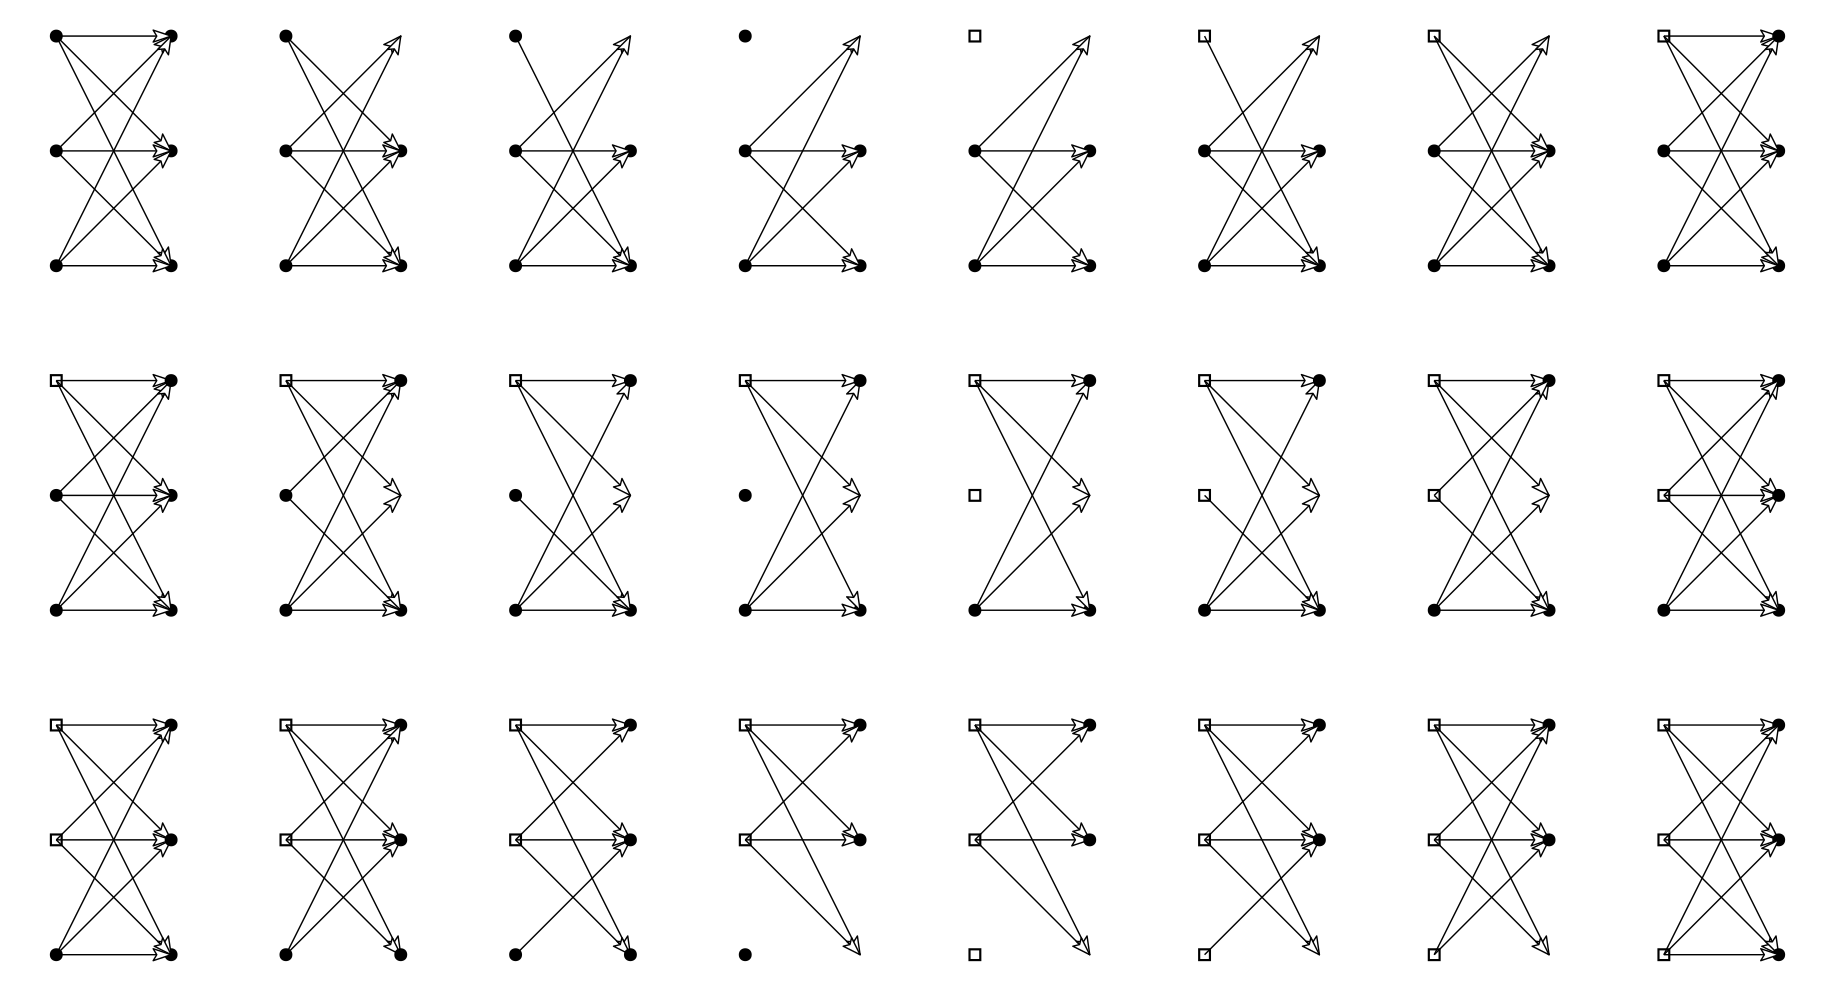
\includegraphics[width=325px]{img/lower_bound_round_proof}
	\caption{Bevis for $t=1$ og $n=3$ \label{lower_bound_round_proof}}
\end{figure}
\newpage
\section{Asynchronous Agreement}
\subsection{Disposition}
\begin{enumerate}
	\item Asynchronous model
  \begin{itemize}
  	\item Ingen tid
    \item Igen øvre grænse
  \end{itemize}
  \item Asynchronous Byzantine Agreement
  \begin{itemize}
    \item Input og output
  	\item Krav
  \end{itemize}
  \item Graded Agreement
  \begin{itemize}
  	\item Udvidelse af weak agreement
    \item Input og output
    \item Krav
    \item Protokol
  \end{itemize}
  \item From Graded Agreement to Terminating Agreement
  \begin{itemize}
  	\item Terminering og time capsuel
    \item Definition 
    \item Protokol
  \end{itemize}
  \item Imposibility of Deterministic Agreement
  \begin{itemize}
  	\item Umuligt med sæt af størrelse 1
    \item Sekvens af operationer på sæt af størrelse 2
    \begin{itemize}
    	\item Umuligt for 2 parties 
      \item Umuligt for 1 party
    \end{itemize}
  \end{itemize}
\end{enumerate}
\newpage

\subsection{Asynchronous model}
\begin{itemize}
	\item Processen $\mathsf P$ har ikke ure 
  \item Protokollerne kan ikke spørge parties til at gøre ting på bestemte tider 
  \item Der er ingen øvre grænse for hvor lang tid, det tager at sende en besked 
  \item Det er antaget, at hvis en besked er sendt af en korrekt proces og processen aldrig crasher, at beskeden eventually bliver delivered 
  \item Delivery er modeleret på følgende måde    
  \begin{itemize}
  	\item Der er en værdi $\Delta_\text{SEND}$
    \item Hvis en besked er sendt er den leveret indenfor dette bound 
    \item Denne bound er ikke kendt af processerne
    \item Den kan være arbitrær stort
  \end{itemize}
  \item Den er nemt at implementere
  \item Svær at bruge
\end{itemize}

\subsection{Asynchronous Byzantine Agreement}
\begin{itemize}
  \item Ethvert Byzantine agreement bliver identificer af en fresh identifier $baid$   
  \item Alle parties kan få input på formen $(\text{VOTE}, baid, v_i)$ hvor $v_i \in \{0,1\}$ bliver kaldt en stemme
  \item Alle parties kan give et output $(\text{DECISION}, baid,d_i)$ hvor $d_i \in \{0,1\}$ bliver kaldt en afgørelse
  \item Krav
  \begin{itemize}
	  \item \textbf{Agreement:} Hvis for en $baid$ nogle korrekt $\mathsf P_i$ og $\mathsf P_j$ outputter $(\text{DECISION}, baid,d_i)$ og $(\text{DECISION}, baid,d_j)$, så gælder der $d_i = d_j$ 
    \item \textbf{Validity:} Hvis for en $baid$ en korrekt $P_i$ giver output $(\text{DECISION}, baid,d_j)$, så har et korrekt party på et tidspunkt har input $(\text{VOTE}, baid, d_i)$
    \item \textbf{Termination:} Hvis for en $baid$ alle korrekte process fik en input på form  $(\text{VOTE}, baid, \cdot)$, så ville alle korrekt processor på et tidspunkt give et output form $(\text{DECISION}, baid, \cdot)$ 
  \end{itemize}
  \item Det er umuligt at lave en deterministisk protokol, der kan håndtere en crash silent error for Byzantine agreement 
\end{itemize}

\subsection{Graded Agreement}
\begin{itemize}
	\item Graded agreement er en udvidelse af weak agreement 
 	\item Der er to mulige outputs for et afgørelse $d_i \in \{0, 1\}$  
  \begin{itemize}
    \item $(d_i,1)$ og $(d_i,2)$
    \item En beslutning med grade 2 betyder, at alle parties har valgt samme beslutning
    \item Hvis outputtet er $?$ så er graden altid $0$  
  \end{itemize}
  \item Syntaksen er på følgende måde 
  \begin{itemize}
  	\item Parties kan have et input på formen $(\text{VOTE}, baid, v_i)$ hvor $baid$ er en ny BA identifier og $v_i \in \{0,1\}$ er en stemme
	  \item Parties kan give output på form $(\text{DECISION}, baid, d_i, g_i)$, hvor $d_i \in \{0,?,1\}$ er en beslutning $g_i \in \{0,1,2\}$ er en karakter 
  	\item Alle mulige output er givet et numre i forhold til den ordende list 
  \begin{equation*}
    n(0,2) = 1, n(0,1) = 1, \dots, n(1,2) =5 
  \end{equation*}
  \end{itemize}
  \item Krav:
  \begin{itemize}
  	\item \textbf{Graded Agreement:} Hvis for en $baid$ to korrekte processer $\mathsf P_i$ og $\mathsf P_j$ outputte $(\text{DECISION}, baid,d_i, g_i)$ og beslutning $(\text{DECISION}, baid,d_j, g_j)$, så $|n(d_i,g_i) - n(d_i,g_i)| \leq 1$
    \item \textbf{Validity:} Hvis en korrekt proces $\mathsf P_i$ outputter $(\text{DECISION}, baid,d_j, g_i)$ hvor $g_i \ne 0$ så havde en korrekt process på et tidligere input $(\text{VOTE}, baid, d_i)$
    \item \textbf{Termination:} Hvis for en $baid$ alle korrekte processor fik input på form $(\text{VOTE}, baid, \cdot)$, så vil alle korrekt processorer eventually give et output på form $(\text{DECISION}, baid,d_i, g_i)$ 
    \item \textbf{Detection:} Hvis for en $baid$ og $v$ alle korrekte processorer fik et input på form $(\text{VOTE}, baid, v)$ så vil alle korrekt processor eventually give et output på form \\ $(\text{DECISION}, baid, v, 2)$ 
  \end{itemize}
  \item Følgende er en protokol, der virker for $n > 9t$
  \begin{enumerate}
  	\item Alle $\mathsf P_i$: Bracha broadcast $v_i$ til alle andre parties 
  	\item Alle $\mathsf P_i$: Vent for $v_j$ fra $n-t$ parties. Lad $V_1$ være antallet af stemmer for $1$. Afhængig af intervallet $I$ som $V_1$ er i set beslutning og karakteren som følgende   
    \begin{itemize}
    	\item Hvis $V_1 \in [0,t]$, så $d_i=0$ og $g_i = 2$ 
    	\item Hvis $V_1 \in (t,3t]$, så $d_i=0$ og $g_i = 1$ 
    	\item Hvis $V_1 \in (3t,n-4t]$, så $d_i=?$ og $g_i = 0$ 
    	\item Hvis $V_1 \in [n-4t,n-2t]$, så $d_i=1$ og $g_i = 1$ 
    	\item Hvis $V_1 \in [n-2t,n-t]$, så $d_i=1$ og $g_i = 2$ 
    \end{itemize}
  \end{enumerate}
  \item Alle der har $d_i = ?$ vælg en ny stemme $0,1$ tilfældig, og dermed konvergerer det imod et fælles svar se Figur~\ref{grade_diagram}
  \begin{itemize}
  	\item Protokollen varer derfor en eller to runder indtil den kommer ind i en af ydre knuderne  
  \end{itemize}
\end{itemize} 
\begin{figure}[h]
	\centering
	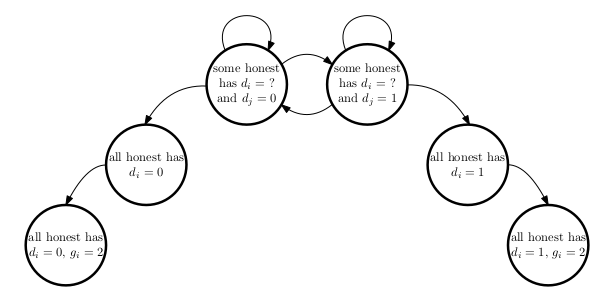
\includegraphics[width=300px]{img/grade_diagram}
	\caption{Graded Agreement votes transformation\label{grade_diagram}}
\end{figure}

\subsection{From graded agreement to Terminating agreement}
\begin{itemize}
	\item Man vil gerne kunne terminere en processen
  \begin{itemize}
  	\item Dette er potentielt farligt at terminere alle sub-protokoler siden en korrekt process $\mathsf P_j$ måske er arbitrært  langt bagefter
    \item Hvis process $\mathsf P_i$ terminere før $\mathsf P_j$ ``vågner op'', så vil $\mathsf P_i$ ikke kunne deltage i den subprotokol 
  \end{itemize}  
  \item Måden man løser dette på er, at sende beskeder der senere vil informere langsomme korrekt processer omkring resultatet af computation når de vågner op     
  \begin{itemize}
  	\item Man kalder dette \textbf{time capsule messages}
    \item De bliver sendt før en party $\mathsf P_i$ terminere
    \item De er der, så kan blive taget op af $\mathsf P_j$, når den vågner op
  \end{itemize}
  \item \textbf{Definition (Asynchronous Termination)} Nå man siger at et party terminere, betyder det partiet terminere dens egen process, sammen med processerne en subprotokol har startet. Der er en vigtig untagelse, den bliver ved med at køre processen, der implementere de authenticated channels den bruger 
  \begin{itemize}
    \item Dette kunne gøres ved at have computerens operativsystemet håndter sendelse og modtagelse af beskeder  
    \item Når en korrekt process terminere har det ikke en effekt på liveness på den protokol der deltog i 
  \end{itemize}
  \item Den følgende protokol antager en protkol for Graded Byzantine Agreement of implementere Byzantine Agreement with Asynchronous Termination. Den virker hvis $n > 3t$ og hvis Graded BA er sikker for de samme $t$ og $n$ 
  \begin{enumerate}
  	\item $\mathsf P_i:$
    \begin{itemize}
    	\item Lad $v_i^0 = v_i$
      \item Lad $r=0$
      \item Lad $\mathsf{GaveOutput} = \bot$  
    \end{itemize}
    \item $\mathsf P_i:$ Kør Graded BA med input $v_i^r$ 
    \begin{itemize}
      \item Lad outputtet være $(d_i^r, g_i^r)$ 
    \end{itemize}
    \item $\mathsf P_i:$ Hvis $d^r_i \ne ?$, sæt $v_i^{r+1} \leftarrow d_i^r$ 
    \item $\mathsf P_i:$ Hvis $d^r_i = ?$, sæt $v_i^{r+1}$ til at være en tilfældig bit 
    \item $\mathsf P_i:$ Hvis $g_i^r=2$ output $(\text{DECISION}, baid, d)$, lad $\mathsf{GaveOutput} = \top$ og send $(\mathsf{TIMECAP}, d)$ til alle parties
    \item Lad $r \leftarrow r+1$ og gå til step 2
  \end{enumerate} 
  \item Udover de andre regler, så kører parties også de følgende ekstra regler
  \begin{itemize}
  	\item \textbf{Term 1} Når man modtager $(\mathsf{TIMECAP}, d)$ fra $t+1$ parties, send $(\mathsf{TIMECAP}, d)$ til alle parties
    \begin{itemize}
    	\item Hvis $\mathsf{GaveOutput} = \bot$ set $\mathsf{GaveOutput} = \top$ og output $(\mathsf{DECISION}, baid, d)$
  \end{itemize}
      \item \textbf{Term 2} Når man modtager $(\mathsf{TIMECAP}, d)$ fra $2t+1$ parties, terminer
  \end{itemize}
\end{itemize} 

\subsection{Impossibility of Deterministic Agreement}
\begin{itemize}
	\item Vi vil gerne bevise, at der ikke eksisterer en deterministisk protokol for Asynchronous Byzantine Agreement, der kan håndtere en enkelt crash-stop error 
  \item Lad $s$ være en scheduling sekvens
  \begin{itemize}
  	\item Altså en sekvens af kommandoer på form $c_1, c_2, c_3, \dots$, hvor hver $c_i$ er en kommando eksekveret men protokolen køre
    \item En kommando $c_i$ kan være noget ligende ``lever beskeden med message identifier $mid$'', ``crash party $\mathsf P_i$'' eller ``schedule party $\mathsf P_j$ 
  \end{itemize}
  \item Beviset tager udgangspunkt i $n=4$ parties, men det holder for et hvilket som helst $n$  
  \begin{itemize}
  	\item Hver $\mathsf P_i$ har et vote $v_i$ 
    \item Vektoren $\pmb v = (v_1, v_2, v_3, v_4)$ 
  \end{itemize}
  \item Tag en hvilket, som helts protokol der opnår Byzantine agreement for fire parties  
  \begin{itemize}
  	\item For en input $\pmb v$ lad $V(\pmb v) \subseteq \{0,1\}$ være sættet af værdier parties måske outputter på de inputværdier  
    \item Der måske mere end en værdi
    \item Outputtet afhænger af hvem der er crashed og i hvilket orden beskederene er scheduled
    \item Vi ved at $V(\pmb v) \ne \emptyset$ 
  \end{itemize}
  \item Vi ved pr. validity at   
  \begin{equation*}
    V(0,0,0,0) = \{0\}
  \end{equation*}
  og
   \begin{equation*}
    V(1,1,1,1) = \{1\}
  \end{equation*}
  \item Nu spørges der hvad $V$ værdierne er for de andre inputs
  \begin{align*}
    V(0,0,0,0) &= \{0\} \\
    V(1,0,0,0) &= \ ? \\
    V(1,1,0,0) &= \ ? \\
    V(1,1,1,0) &= \ ? \\
    V(1,1,1,1) &= \{1\} 
  \end{align*}
  \item Der argumenteres nu for at en af dem skal være $\{0,1\}$. Antag at dette ikke er tilfældet
  \begin{itemize}
  	\item Dette betyder, at alle sæt har størrelse 1
    \item Det betyder, at der er sted hvor outputtet skifter fra $\{0\}$ til $\{1\}$
    \item Antag uden loss of generality, at det her er 
    \begin{align*}
      V(1,1,0,0) &= \ \{0\} \\
      V(1,1,1,0) &= \ \{1\} \\
    \end{align*}
    \item Overvej følgende eksekvering af $\pi$ på input $(1,1,0,0)$  
    \begin{enumerate}
    	\item Crash $\mathsf P_3$  
      \item Kør i forhold til en hvilken som helst message schedule 
      \item Siden antagelsen er at $V(1,1,0,0) = \ \{0\}$, så kan outputtet kun være $0$ 
    \end{enumerate}
    \item Overvej følgende eksekvering af $\pi$ på input $(1,1,1,0)$  
    \begin{enumerate}
    	\item Crash $\mathsf P_3$  
      \item Kør i forhold til en hvilken som helst message schedule 
      \item Siden antagelsen er at $V(1,1,1,0) = \ \{1\}$, så kan outputtet kun være $1$ 
    \end{enumerate}
    \item Siden $\mathsf P_3$ crasher i begge situation, så kan outputtet ikke afhænge af dette og siden de outputter to forskellige ting er dette en modstrid. 
  \end{itemize} 
  \item Derfor må der være et input, der giver en $V$ værdi $\{0,1\}$  
  \begin{itemize}
  	\item Antag uden loss of generality, at det er 
    \begin{equation*} 
      V(1,1,0,0) = \ \{0,1\} 
    \end{equation*}
    \item Lad $s$ være en scheduling sequence  
    \begin{itemize}
    	\item Et tal skrift i protkolen, der siger hvilken besked man skal leveres næst 
      \item Lad
      \begin{equation*} 
        V(1,1,0,0, s) \subseteq \{0,1\} 
      \end{equation*}
      være de værdi protokollen kan outputte efter først kører med hensyn til $s$ også køre en hvilken som helst sekvens af kommandoer dernæst 
    \end{itemize}
    \item Siden at protokollen terminere for en lang nok sekvens $s$ holder det at 
    \begin{equation*}
      V(1,1,0,0, s) = \ \{0\} \\
    \end{equation*}
    eller 
    \begin{equation*}
      V(1,1,0,0, s) = \ \{1\} \\
    \end{equation*}
    \item Vi ved, at for den tomme sekvens $\epsilon$, at der gælder
    \begin{equation*}
      V(1,1,0,0, \epsilon) = \ \{0, 1\} \\
    \end{equation*}
    \item Derfor må der eksisterer en maksimal sekvens $s$, så uanset hvilken commando $d$, der bliver appended til $d$, så vil det holde at 
    \begin{equation*}
      V(1,1,0,0, (s,d)) = \ \{0\} \\
    \end{equation*}
    eller 
    \begin{equation*}
      V(1,1,0,0, (s,d)) = \ \{1\} \\
    \end{equation*}
    \item Der må eksisterer deliveries $d_0$ og $d_1$ sådan at   
    \begin{equation*}
      V(1,1,0,0, (s,d_0)) = \ \{0\} \\
    \end{equation*}
    eller
    \begin{equation*}
      V(1,1,0,0, (s,d_1)) = \ \{1\} \\
    \end{equation*}
    \item Antag $d_0$ er en delivery til $\mathsf P_i$ og $d_1$ er en delivery til $\mathsf P_j$. Dermed hvis man først eksekvere $d_0$ også $d_1$ eller den anden vej rund have samme effekt så
    \begin{equation*}
      V(1,1,0,0, (s,d_0,d_1)) = V(1,1,0,0, (s,d_1,d_0)) \\
    \end{equation*}
    hvilket er en klar modstrid
    \item Den eneste mulighed er, at de er leveret til samme $\mathsf P_i$
    \begin{itemize}
    	\item Det kommer til at afhænge af rækkefølgen beskederne kommer i
      \item Det kan ikke lade sig gøre, siden hvis $\mathsf P_i$ crasher før har kan fortælle det til resten af netværket kan resten ikke vælge den rigtig beslutning
      \item Formelt lad $c_i$ være en scheduling, der starter med at crashe $\mathsf P_i$. Derfor må der gælde
    \begin{equation*}
      V(1,1,0,0, (s,d_0,c_i)) = V(1,1,0,0, (s,d_1,c_i)) \\
    \end{equation*}
    hvilket er en klar modstrid
    \end{itemize}
  \end{itemize}
\end{itemize} 
\newpage

\section{State-Machine Replications}
\subsection{Disposition}
\begin{enumerate}
	\item State Machine
  \begin{itemize}
  	\item Definition
  \end{itemize}
	\item Replicated State Machine 
  \begin{itemize}
  	\item Definition
    \begin{itemize}
    	\item Syntaks
      \item Idel funktionalitet
    \end{itemize}  
    \item Liveness og safety property
  \end{itemize}
	\item Totally Ordered broadcast 
  \begin{itemize}
  	\item Definition
    \begin{itemize}
    	\item Syntaks
      \item Idel funktionalitet
    \end{itemize}  
    \item RSM fra TOB
    \item Syncronous Implementation
  \end{itemize}
\end{enumerate}
\newpage

\subsection{State Machine}
\begin{itemize}
	\item \textbf{Definition} En \textbf{state machine} $M$ består af  
  \begin{itemize}
  	\item Et sæt $\mathsf{States}$
    \item En start state $\mathsf{State}_0 \in \mathsf{States}$
  	\item Et sæt $\mathsf{Inputs}$
  	\item Et sæt $\mathsf{Outputs}$
  	\item En transitionsfunktion $T: \mathsf{States} \times \mathsf{Inputs} \to \mathsf{States} \times \mathsf{Outputs}$ 
    \item En state machine starter i $\mathsf{State}_0$
    \begin{itemize}
	    \item Når den er i tilstand $\mathsf{State}_i$ og modtager input $x$ udregner den $(State_{i+1},y)=T(\mathsf{State}_i,x)$, og ændre tilstanden til $\mathsf{State}_{i+1}$ og outputter $y$ 
    \end{itemize} 
  \end{itemize}
\end{itemize}

\subsection{Replicated State Machine}
\begin{itemize}
	\item En replicated state machine er en protocol for $n$ serverer, der får dem til at opfører sig som om de kun er en enkelt state machine $M$ 
  \item \textbf{Definition} Lad $M$ være en state machine. En \textbf{replicated state machine} er specificeret vha. en ideal funktionalitet $\mathsf{RSM}_M$ for $n$ servers $\mathsf{S}_1, \dots, \mathsf{S}_n$
  \begin{itemize}
	  \item Syntaksen er på følgende måde
    \begin{itemize}
  		\item Der er en protokol port $\mathsf{IO}_i$ der modtager input fra server $\mathsf{S}_i$ og giver outputs fra server $\mathsf{S}_i$
  		\item Der er en speciel port $\mathsf{RECEIVED}_i$, der reporter hvilke beskeder der er blevet inputtet til den idelle funktionalitet af $\mathsf{S}_i$
  		\item Der er en speciel port $\mathsf{PROCESS}$, der specificere hvilke beskeder der skal processers næste gange 
  		\item Der er en speciel port $\mathsf{DELIVER}_i$ der instruere den idele funktionalitet til at levere den næste besked til $\mathsf{S}_i$ 						
    \end{itemize}
  	\item Den idelle funktionalitet kører på følgende måde: 
    \begin{itemize}
    	\item Intialisering 
      \begin{itemize}
			  \item Lad $\mathsf{State}=\mathsf{State}_0$
  			\item For hver $\mathsf{IO}_i$, lad $Q_i$ være den tomme kø: $Q_i$ er outputs for serveren $\mathsf S_i$ der ikke er blevet leveret endnu
  			\item Initialisere $\mathsf{UnProcessed}$ til at være det tomme sæt
      \end{itemize}
		\item På input $x$ til $\mathsf{IO}_i$, output $x$ på $\mathsf{RECEIVED}_i$ og tilføj $x$ til $\mathsf{Unprocessed}$
		\item På input $x$ til $\mathsf{PROCESS}$ hvor $x \in \mathsf{UnProcessed}$
    \begin{enumerate}
			\item Lad $(\mathsf{State}', y)=T(\mathsf{State},x)$ og opdatere $\mathsf{State}= \mathsf{State}'$
			\item Tilføj $y$ til alle køer $Q_i$
			\item Fjern $x$ fra $\mathsf{UnProcessed}$
    \end{enumerate}
		\item På input til $\mathsf{DELIVER}_i$ hvor $Q_i$ ikke er tom, fjern det første element $y$ fra $Q_i$ og output $y$ på $\mathsf{IO}_i$
    \end{itemize}
  \end{itemize}
  \item En vigtig liveness property er, at hvis $x$ bliver tilføjet til $\mathsf{UnProcessed}$, at så må den eventually blive processerede og alle outputs vil eventually blive leveret
  \item En vigtig safety property er at alle outputs partierne ser er altid resultatet af at køre fra en initel tilstand på en sekvens af de samme inputs for alle parties 
  \begin{itemize}
  	\item Parties der bruger $\mathsf{RSM}_M$ har måske ikke set de samme antal outputs
  \end{itemize}
\end{itemize}

\subsection{Totally ordered broadcast}
\begin{itemize}
	\item En vigtig del af implementationen af state-machine replication er totally-ordered broadcast
  \item \textbf{Definition} Opførelsen af totally ordered broadcast er beskrevet via den ideelle funktionalitet $\mathsf{TOB}$ for $n$ parties $\mathsf P_1, \dots, \mathsf P_n$ 
  \begin{itemize}
  	\item Syntaksen er som følger
    \begin{itemize}
    	\item Der er en protokol port $\mathsf{IO}_i$ til at modtage inputs fra server $\mathsf{P}_i$ og giver outputs til $\mathsf{P}_i$ 
  		\item Der er en speciel port $\mathsf{RECEIVED}_i$, der reporter hvilke beskeder der er blevet inputtet til den idelle funktionalitet af $\mathsf{S}_i$
  		\item Der er en speciel port $\mathsf{QUEUE}$, der specificere hvilke beskeder, der skal queues næste gang  
  		\item Der er en speciel port $\mathsf{DELIVER}_i$ der instruere den idele funktionalitet til at levere den næste besked til $\mathsf{S}_i$ 						
    \end{itemize}
    \item Den ideelle funktionalitet kører på følgende måde
    \begin{itemize}
    	\item Intialisering
      \begin{itemize}
      	\item Lad $\mathsf{UnQueued} = \emptyset$
        \item For hver $\mathsf{IO}_I$, lad $Q_i$ være den tomme kø
        \item Køen $Q_i$ er outputs for $\mathsf P_i$ som endnu ikke er blevet leveret
      \end{itemize}
      \item På input $x$ på $\mathsf{IN}_i$ output $x$ på $\mathsf{RECEIVED}_i$ og tilføj $x$ til $\mathsf{UnQueued}$ 
      \item På input $x$ på $\mathsf{QUEUE}$ hvor $x \in \mathsf{UnQueued}$, læg $x$ ind i alle køer $Q_i$ og fjern $x$ fra $\mathsf{UnQueued}$ 
      \item På et input på $\mathsf{DELIVER}_i$, hvor $Q_i$ ikke er tom, fjern det første element $x$ fra $Q_i$ og output $x$ på $\mathsf{IO}_i$ 
    \end{itemize}
  \end{itemize}
  \item Replicated State Machine for $M = (\mathsf{States}, \mathsf{State}_0 , \mathsf{Inputs}, \mathsf{Outputs})$ fra Totally-Ordered Broadcast
  \begin{itemize}
  	\item Protokollen har $n$ servere $\mathsf {S}_i$ og bruger $\mathsf{TOB}$ 
    \begin{itemize}
    	\item Hver $\mathsf{S}_i$ har en port $\mathsf{RSM}_M.\mathsf{IO}_i$ for at modtage inputs og give output til $P_i$  
      \item Hver $\mathsf{S}_i$ har en port der er forbundet til $\mathsf{TOB}.\mathsf{IO}_i$ så den kan give $\text{TOB}$ inputs og outputs
    \end{itemize}
    \item Protokollen kører på følgende måde
    \begin{itemize}
    	\item $\mathsf{S}_i$: Initialisering: initialisere $\mathsf{TOB}$ og lad $\mathsf{State} = \mathsf{State}_0$ 
    	\item $\mathsf{S}_i$: På input $x$ på $\mathsf{RSM}_M.\mathsf{IO}_i$ input $x$ på $\mathsf{TOB}.\mathsf{IO}_i$
    	\item $\mathsf{S}_i$: På output $x$ på $\mathsf{TOB}.\mathsf{out}_i$ lad $(\mathsf{State}', y) = T(\mathsf{State}, x)$, opdaterer $\mathsf{State} = \mathsf{State}'$ og output $y$ på $\mathsf{IO}_i$ 
    \end{itemize}
  \end{itemize}
\end{itemize}

\subsubsection{Synchronous Implementation}
\begin{itemize}
	\item En sequencer bliver valgt i hver runde 
  \begin{itemize}
  	\item Den vælger broadcaster en block, som er rækkefølgen i den runder for beskeder
    \item Hvis sequenceren er korrupt kan den ødelægge liveness ikke safety siden, at de kun kan lade hver med at vælge en rækkefølge 
    \begin{itemize}
    	\item De kan også tilføje en ikke eksisterende $x$ rækkefølgenden, men dette er ikke et attack siden de kunne opnå det samme ved at broadcaste det
    \end{itemize}
  \end{itemize}
\end{itemize}
\begin{framed}  
  \begin{center}  
     \textbf{Synchronous Totally-Ordered Broadcast}
  \end{center}
  \begin{itemize}
  	\item En protokol for $n$ parties $\mathsf{P}_1, \dots, \mathsf{P}_n$ bruger
    \begin{itemize}
    	\item En unscheduled consensus broadcast $\mathsf{UCB}$ 
      \item En scheduled consesus broadcast, hvor alle korrekt parties terminere i samme runde $\mathsf{SCB}$  
    \end{itemize}
    \item Den første del af protokollen bruger følgende activation regler 
    \begin{itemize}
    	\item $\mathsf{P}_i$: På input $x$ på $\mathsf{TOB}.\mathsf{IO}_i$ input $x$ på $\mathsf{UCB}.\mathsf{IO}_i$
      \item $\mathsf{P}_i$: På output $x$ på $\mathsf{UCB}.\mathsf{IO}_i$ tilføj $x$ til $\mathsf{UnQueued}_i$ 
    \end{itemize}
    \item Den anden del af protokollen bruger følgende activation regler 
    \begin{enumerate}
    	\item Initialisering:
      \begin{itemize}
        \item Lad $\mathsf{UnQueued}_i = \emptyset$ og $\mathsf{Queued}_i = \emptyset$ 
        \item Lad $\mathsf{epoch} = 1$ 
        \item Værdien $\mathsf{epoch}$ indikere hvem lederen er i et given epoch
        \item Lederen i epoch $\mathsf{epoch}$ er $\mathsf{P}_i$ hvor $i=\mathsf{epoch}$ 
      \end{itemize}
      \item Gør følgende
      \begin{itemize}
        \item Leder $\mathsf{P}_i$: Lad $U_i = \mathsf{UnQueued}_i \backslash \mathsf{Queued}_i$ og input $U_i$ på $\mathsf{SCB}.\mathsf{IN}_i$ 
        \item $\mathsf{P}_{j \ne i}$ Input $P_i$ på $\mathsf{SCP}.\mathsf{IN}_j$ for at indikere at $P_i$ broadcaster 
      \end{itemize}
      \item Når er block $U$ er modtaget på $\mathsf{SCB}.\mathsf{OUT}_j$ gør følgende
      \begin{enumerate}
      	\item Fjern $U$ fra $\mathsf{UnQueued}_i$  
        \item Tilføj $U$ to $\mathsf{Queued}_i$ 
        \item Output på $\mathsf{TOB}.\mathsf{OUT}_j$ elementerne i $U$ i deterministisk orden e.g. lexicographically 
        \item Lad $\mathsf{epoch}=\mathsf{epoch} +1$ 
        \item Gå til step 2 
      \end{enumerate}
    \end{enumerate}
  \end{itemize}
\end{framed}

\newpage

\section{Blockchains, How to grow a tree}
\subsection{Disposition}
\begin{enumerate}
	\item Blockchains
  \begin{itemize}
  	\item Definition
    \item Tid
    \item Flooding system
  \end{itemize}
  \item Lottery System
  \begin{itemize}
  	\item Lottery system
    \item Draw, value og tickets
    \item Unik vinder
    \item Protokol
    \begin{itemize}
    	\item Hardness  
      \item Block definition
      \item Genesis block
      \item Ath weight
      \item Best path
      \item Protokol
    \end{itemize}
  \end{itemize}
  \item Properties
  \begin{itemize}
    \item Standard tree scenario
    \item Honest tree
  	\item Tree growth
    \item Chain quality
    \item Limited rollback
  \end{itemize}
  \item Finalisation problem
\end{enumerate}
\newpage

\subsection{Blockchains}
\begin{itemize}
	\item En \textbf{blockchain} er en implementation af totally ordered broadcast og kan blive brugt alle steder, hvor et totally ordered broadcast er brugbart
  \begin{itemize}
  	\item Dette kun fx være state machine replication
    \item En \textbf{cryptocurrency} er et lag, som kan blive lagt oven på enhver totally-ordered broadcast 
  \end{itemize}
  \item Der bliver antaget en global fysisk time $t$ 
  \begin{itemize}
  	\item Hver party har et lokalt ur $\mathsf{Clock}_i$ 
    \item En begrænsning $\mathsf{MaxDrift}$ bliver antaget på ur drift
    \begin{itemize}
    	\item Det er antaget at $|t-\mathsf{Clock}_i| \leq \mathsf{MaxDrift}/2$ for alle korrekt $\mathsf{P}_i$ 
      \item For to korrekte $\mathsf{P}_i$ og $\mathsf{P}_j$ vil den følgende relation være opfyldt $|\mathsf{Clock}_i - \mathsf{Clock}_j \leq \mathsf{MaxDrift}$ 
      \item Dette kan fx opnås ved at synkronisere med en server
    \end{itemize}
  \end{itemize}
  \item Det er antaget, at der er et flooding system 
  \begin{itemize}
  	\item En model er overvejet, hvor parties kan komme og gå
    \item Hvis et party er vågen, når en besked er sendt og bliver vågen i lang nok tid, så får den med garanti beskeden 
    \item Der er en fast øvre grænse $\mathsf{MaxDeliverytime}$ på delivery tiden
  \end{itemize}
  
\end{itemize}

\subsection{Lottery Systems - Proof of Stake}
\begin{itemize}
	\item Et lottery system $\mathsf{LOTTERY}$ er antaget
  \begin{itemize}
    \item Den deler tiden ind i $\mathsf{slots}$ af længde $\mathsf{SlotLength}$ 
    \item Et party $\mathsf{P}_i$ et i slot $\mathsf{slot}$ hvis
  \begin{equation*}
    \mathsf{slot}-1 \leq \frac{\mathsf{Clock}_i}{\mathsf{SlotLength}} < \mathsf{slot}
  \end{equation*}
  \end{itemize}
  \item Lottery systemet lader et party $\mathsf{P}_i$ få et draw $\mathsf{Draw}_{i,\mathsf{slot}}$ for hver slot
  \begin{itemize}
  	\item Ethvert draw har en associerede værdi $\mathsf{Val}(\mathsf{Draw}_{i,\mathsf{slot}})$  
    \item Vinderen i et given slot er det party med højeste $\mathsf{Val}(\mathsf{Draw}_{i,\mathsf{slot}})$
    \item Hver party har en associerede værdi $\mathsf{Tickets}_i$, der er kendt af alle parties
    \begin{itemize}
    	\item I proof of stake systemer svarer dette typisk, til hvor mange penge der er på kontoen 
    \end{itemize}
    \item Hvert party generer i første runde et nøglepar $(\mathsf{vk}_i, \mathsf{sk}_i)$ for et signature scheme
    \begin{itemize}
    	\item Den sender $\mathsf{vk}_i$ til alle andre parties
      \item Signature schemet skal have unikke signature  
    \end{itemize}
    \item I anden runde bliver et tilfældigt tal $\mathsf{Seed}$ gjort offentligt 
    \begin{itemize}
    	\item Det er vigtigt, at dette ikke er kendt i runde 1 
    \end{itemize}
    \item For hver $slot = 0,1,\dots,$ party $\mathsf{P}_i$ kan udregne draw 
    \begin{equation*}
      \mathsf{Draw}_{i,\mathsf{slot}} = \mathsf{Sig}_{\mathsf{sk}_i}(\mathsf{LOTTERY}, \mathsf{Seed}, \mathsf{slot}) 
    \end{equation*}
    \item Værdien af et draw er defineret som følger: Hvis $\mathsf{Ver}_{\mathsf{vk}_i}(Draw,(Lottery, Seed, slot)) = \bot$, så $\mathsf{Val}(\mathsf{P}_i,\mathsf{slot}, \mathsf{Draw}) = - \infty$ ellers 
    \begin{equation*}
      \mathsf{Val}(\mathsf{P}_i,\mathsf{slot}, \mathsf{Draw}) = \mathsf{Tickets_i} \cdot H(\mathsf{LOTTERY}, \mathsf{Seed}, \mathsf{slot}, \mathsf{P}_i, \mathsf{Draw})
    \end{equation*}
    Funktionen $H$ er en kryptografisk hash funktion med 256 bit output   
  \end{itemize}
  \item Alle parties kan udregne $\text{Val}(P_i, \text{slot}, \text{Draw})$ for alle $P_i,\text{slot}, \text{Draw}$
  \begin{itemize}
  	\item Grunden til at man skal have en unik signatur for $(\text{LOTTERY}, \text{Seed}, \text{slot})$ er at ellers kan et korrupt party udregne signaturen flere gange og vælge den med højest værdi
  \end{itemize}
  \item Der er en unik vinder i hver runde
  \begin{itemize}
  	\item Outputs af $H$ er antaget at være uniform tilfældig i intervallet $[0,2^{256})$, derfor er der forsvindende lille sandsynligheden for at to parties får samme nummer
    \item For at være helt sikker på at der er en unik vinder, så hvis to parties får samme værdi, sammenlignes deres verifikationsnøgler i stedet for    
  \end{itemize}
\end{itemize}

\subsubsection{Protocol}
\begin{itemize}
	\item Kun parties med en værdi højere end nummeret $\mathsf{Hardness}$ sender deres block
  \begin{itemize}
  	\item Dette sparer meget bandwidth siden, at alle parties ikke længere skal sende noget hver runde
    \item Gør også, at der nogle runder, hvor der er ingen der vinder 
  \end{itemize}
  \item Man gror et træ i stedet for en kæde
  \begin{itemize}
  	\item Dette løser problemet med at det ikke er alle der har set en vindende block
    \item Træet konvergerer typisk imod Agreement 
  \end{itemize}
  \item \textbf{Definition} En knude er på formen $(\text{BLOCK}, \text{P}_j, \text{slot}, \text{Draw}, U,h, \sigma)$
  \begin{itemize}
		\item $\text{BLOCK}$ er typen af tuplen
		\item $\text{slot} \in \mathbb N$ er block nummeret 
		\item $\text{Draw}$ er det draw, der blev brugt til at vinde lotteriet
		\item $U$ er blockdata
		\item $h$ er block hash af den tidligere block
  	\item Værdien af block $N$ er defineret til at være $\text{Val}(N.\text{P}, N.\text{slot}, N.\text{Draw})$
  \end{itemize}
  \item Der er en specielt block $(\text{BLOCK}, \bot, 0, \bot, U_0, \bot)$ med værdi $\infty$ kaldet genesis blokken med, hvor $U_0$ er genesis data
  \begin{itemize}
  	\item Den indeholde $\mathsf{Hadness}$ og mere
    \item Bliver kaldt $G$  
  \end{itemize}
  \item For en givet sæt $S$ af blocks, som indeholder $G$ og hvor alle blokke er valide definere et træ på følgende måde
  \begin{itemize}
    \item Roden er træet er genesis blokken $G$ 
    \item Kanterne er directed og peger imod roden 
		\item Der er en kant $N_1 \in \mathsf{Tree}$ fra $N_2 \in \mathsf{Tree}$ hvis og kun hvis $N_2.h = H(N_1)$ og $N_2.\mathsf{slot} > N_1.\mathsf{slot}$
		\item For en given node $N$ lad $\mathsf{PathTo}(N)$ være listen af noder fra $G$ til $N$ inklusiv $G$ og $N$ indekseret fra 0
  \end{itemize}
	\item En weight er en funktion $\mathsf{PathWeight}$ der mapper blockchains til et tal 
  \begin{itemize}
    \item Det skal gælde at
    \begin{itemize}
  		\item Hvis $P'$ er et proper prefix af $P$, så $\mathsf{PathWeight}(P^{'}) < \mathsf{PathWeight}(P)$ 
  		\item Hvis $P \ne P'$ så $\mathsf{PathWeight}(P') \neq \mathsf{PathWeight}(P)$
  		\item Det kan ikke ske at $\mathsf{PathWeight}(P') < \mathsf{PathWeight}(P)$ og $\mathsf{Len}(\mathsf{PathWeight}(P^{'})) > \mathsf{Len}(\mathsf{PathWeight}(P))$ 
    \end{itemize}
    \item Den $\mathsf{PathWeight}$ man typisk bruger kigger først på længden og dernæst på værdien $\mathsf{Val}(\mathsf{Leaf}(P))$
  \end{itemize}
  \item $\mathsf{BestPath}(\mathsf{Tree})$ er den den path der maksimere $\mathsf{PathWeight}$
  \item Protokollen har to hjælpe funktioner
  \begin{enumerate}
	  \item \texttt{GetMetaData} spørger det lokale system, det ekstra data der er i block data
    \item \texttt{ValidMetaData} tjekker, at dataen er valid 
  \end{enumerate}
\end{itemize}
\begin{framed}  
\begin{center}  
  \textbf{Blockchain protokol} 
\end{center}
\begin{itemize}
	\item $\mathsf{P}_i:$ 
  \begin{itemize}
  	\item Lad $\mathsf{slot}_i$ være det nuværende slotnummer 
    \item Lad $\mathsf{slot}_i=0$ 
    \item Lad $\mathsf{Delivered}_i = \emptyset$  
    \item Lad $\mathsf{Received}_i$ være beskederne modtaget af flooding systemet 
    \item Lad $G$ være geneesis block og til at starte med lad $S_i = \{G\}$  
    \item Igennem protokolen lad $\mathsf{Tree}_i = \mathsf{Tree}(S_i)$ 
  \end{itemize}
  \item Hver $\mathsf{P}_i$ kører følgende activation regler. Alle værdier er sendt via $\mathsf{FLOOD}$  
  \begin{enumerate}
  	\item Når slot $\mathsf{slot}_i$ begynder, lad $P = \mathsf{BestPath}(\mathsf{Tree}_i)$ get draw $\mathsf{Draw}_i$.\\ Hvis $\mathsf{Val}(\mathsf{P}_j,\mathsf{slot}, \mathsf{Draw}) \geq \mathsf{Hardness}$ gør følgende
    \begin{itemize}
    	\item Lad $M_i = \mathsf{GetMetaData}$ 
      \item Lad $U_i = \mathsf{Received}_i \backslash \mathsf{Delivered}_i$ 
      \item Lad $B_i = \mathsf{Leaf}(P)$ 
      \item Lad $h_i = H(B_i)$ 
      \item Lad $\sigma_i = \mathsf{Sig}_{\mathsf{sk}_i}(V_i)$ 
      \item Send $V_i = (\mathsf{BLOCK}, \mathsf{P}_i, \mathsf{slot}_i, \mathsf{Draw}_i, (U_i,M_i), h_i, \sigma_i)$
    \end{itemize}
    \item På input $V_j = (\mathsf{BLOCK}, \mathsf{P}_j, \mathsf{slot}_j, \mathsf{Draw}_j, (U_j,M_j), h_j, \sigma_j)$ hvor $\mathsf{Ver}_{\mathsf{vk}_j}(\sigma_j,V_j) = \top$ og $\mathsf{Val}(\mathsf{P}_j,\mathsf{slot}, \mathsf{Draw}) \geq \mathsf{Hardness}$
    \begin{itemize}
    	\item Gem den og vent ind til at $\mathsf{slot}_i>\mathsf{slot}$ og $\mathsf{ValidMetaData}(M) = \top$ og tilføj det til $S_i$ 
    \end{itemize} 
  \end{enumerate}
\end{itemize}
\end{framed}


\subsection{Properties in Standard Scenario}
\begin{itemize}
	\item I \textbf{standard tree scenario} følgende er antaget
  \begin{itemize}
  	\item Mindst $66\%$ at tickets er honest  
    \item $\mathsf{MaxDeliveryTime}$ gør således at $95\%$ af alle slots er timely
    \item Hardness er således at sandsynligheden for, at der er en slot vinder i et givet slot er $10\%$ 
  \end{itemize}
  \item \textbf{Definition} Givet to valide træer, deres union er igen et valid træ
  \begin{itemize}
    \item Unionen er alle paths, der er i begge træer
  	\item Lad $H$ være sættet af alle valide træer 
    \begin{equation*}
      \text{HonestTree}^t_\text{slot} = \bigcup_{i\in H} \text{Tree}_i^t
    \end{equation*}
    \item Alle korrekt parties ser et subset af det honest tree  
  \end{itemize}
\end{itemize}

\subsubsection{Tree growth}
\begin{itemize}
	\item \textbf{Definition} Lad $\mathsf{TreeGrowth} \in [0,1]$ være et reelt tal. Det siges, at en protokol har en \textbf{tree growth} $\mathsf{TreeGrowth}$, hvis efter $n$ slot winners højden af $\text{HonestTree}$ er mindst $\text{TreeGrowth} \cdot (n-\kappa)$ udover med en meget lille sandsynlighed $2^{-\kappa}$
  \item \textbf{Definition} Et slot $\mathsf{slot}$ er \textbf{timely}, hvis alle beskeder før tid $t-\text{MaxDeliveryTime}$ er leveret før tid $t$ 
  \item \textbf{Definition} Et slot $\mathsf{slot}$ er \textbf{honest slot} hvis der er mindst en honest vinder i slot $\mathsf{slot}$
	\item \textbf{Definition} Et slot $\mathsf{slot}$ er et \textbf{lucky slot} hvis det både er timely og honest 
  \item \textbf{Lemma} Observere et timely slot $\text{slot}$ og lad $\text{HonestTree}^t$ være det honest tree, når slottet begynder
  \begin{itemize}
  	\item Antag at der er en honest winner i slot $\text{slot}$
    \item Lad $\text{HonestTree}^{t-\text{MaxDeliveryTime}}$ være det honest tree $\text{MaxDeliveryTime}$ sekunder før. Så gælder der
  \begin{equation*}
    \text{Len}(\text{BestPath}(\text{HonestTree}^t)) \geq \text{Len}(\text{BestPath}(\text{HonestTree}^{t-\text{MaxDeliveryTime}})) + 1
  \end{equation*}
  \end{itemize}
  \item \textbf{Definition} Et honest slot winner er wasted, hvis der vinder et slot som ikke er timely eller hvis den vinder et timely slot, som har en anden honest vinder med højere værdier  
  \begin{itemize}
    \item Lad $\text{WastedHonestWinners}^t$ være antallet af waster honest vindere til tid $t$
  \end{itemize}
  \item \textbf{Theorem} Lad $\mathsf{HonestWinners}^t$ være antallet af honest vindere til tid $t$. Så gælder det at 
  \begin{equation*}
    \text{Len}(\text{BestPath}(\text{HonestTree}^t)) \geq \text{HonestWinners} ^t -\text{WastedHonestWinners}^t
  \end{equation*}
  \item Der vil være cirka $59\%$ lucky slots med en vinder
  \begin{itemize}
    \item Siden cirka $95\% \cdot 66\% = 63\%$ af slots har mindst en honest vinder og sandsynligheden for at man rammer en, som allerede har en honest vinder er $6.3\%$ er der $63\% \cdot (100\%-6.3\%) = 59\%$ lucky slots med en vinder
    \item Dette betyder at tree grow er $59\%$ 
    \item Der vil være cirka $34\%$ korrupt slots 
  \end{itemize}
\end{itemize}
  
\subsubsection{Chain quality}
\begin{itemize}
  \item \textbf{Definition} Lad $\text{ChainQuality} \in [0,1]$ være et reelt tal. Det siges at en protokol har en \textbf{chain quality} $\text{ChainQuality}$, hvis efter $n$ slot vinderen den bedste path i $\mathsf{HonestTree}$ har $\text{ChainQuality} \cdot L - \kappa$ noder der var produceret af honest parties. Undtagen med en lille sandsynlighed $2^{-\kappa}$ 
  \item Protokollen i det standard tree scenario har en chain quality på cirka $42\%$ 
  \begin{itemize}
  	\item Det har den siden, at hvis der er $n$ vinderer har honest tree en højde på $.59n$ ud af dem er mindst $.59n-.34n=.25n$ honest. Derfor får vi en chain quality på $.25/.34>.42$ 
  \end{itemize}
\end{itemize}

\subsubsection{Limited roll-back}
\begin{itemize}
  \item The limited rollback egenskab siger, at der er en begrænsning $\text{RollbackLimit}$ således at sandsynligheden for at der er rollbacks bag ved den limit er meget lille
  \item \textbf{Definition} \textbf{super slot} er et slot der er blevet vundet af et honest party, hvor slottet var timely og der ikke var andre slots der har vundet den 
  \item \textbf{Lemma} Alle super blocks er på forskellig højder i det honest tree
  \begin{itemize}
  	\item Alle blocks der ikke er super blocks bliver kaldt filler block
  \end{itemize}
  \item \textbf{Lemma} Antag at et rollback er mulig fra branch $B_1$ til branch $B_2$ der begge to har rod $N$. Hvis der siden $N$ var lavet er blevet lavet $s$ super blocks, så var der mindst $s/2$ filler blocks lavet
  \item Hvis man skal have en ordenlig sikkerhed skal man kunne tollere rollback af længde 40  
\end{itemize}

\subsection{Lack of finality problems}
\begin{itemize}
	\item Et stor problem med tree protokoler er, hvornår man skal gennemføre en transaction 
  \begin{itemize}
  	\item Hvis man vil undgå rollbacks, kan parties ikke deliver en transaction på $\text{IO}_i$, der måske bliver roolback
  \end{itemize}
  \item Der er to forskellig løsninger til dette problem 
  \begin{enumerate}
  	\item Vent lang nok tid og en block er kun sikker når den er lang nok oppe i træet 
    \item Kør en seperat process der afgør når en block er final, hvilket bliver kaldt finalization layer
  \end{enumerate}
\end{itemize}

\newpage

\end{document}
%%% Local Variables:
%%% mode: latex
%%% TeX-master: t
%%% End:

